\chapter{线性多自由度系统}

上一章中，我们从做一维运动，或可简化为做一维运动的质点出发，广泛介绍了常见的一维问题和所对应的数值算法。然而，实际的物理问题中往往存在着多个，甚至是无穷多个相互耦合的自由度，这些高维问题同样需要我们发展有效的数值计算手段来处理。作为起点，本章中我们便尝试接触其中最简单的部分：线性多自由度系统。

所有的线性多自由度系统的求解归根结底都可以划归成两类问题：线性代数方程组与本征值问题。在本章中，我们将介绍处理这两类问题的数值算法。

\section{电路网络：线性代数方程组的直接解法}

从跨越大江大河、高山峡谷的高压输电网络，到雕刻于纳米芯片上的集成电路，人们通过制造和组合大量的元器件，设计电路网络，让电实现各种各样的功能。为了理解和掌握这些各式各样的电路，我们需要知道如何求解其中的电势和电流分布。

对于仅由线性元件所构成的电路网络，这个问题可以转化为一个线性代数方程组的求解。我们用指标 $i=1,2,\ldots,n$ 标记电路网络中的各个节点，$i,j$ 两节点之间直连的电导记作 $g_{ij}$，接入的电压源记作 $\epsilon_{ij}$，对于断路的情形 $g_{ij}=0$。记节点 $i$ 的电势为 $U_i$，那么由节点 $i$ 直接流向 $j$ 的电流为
\begin{equation}
g_{ij}(U_i-U_j+\epsilon_{ij}).
\tag{3.1.1}
\end{equation}
根据 Kirchhoff 第一定律（电流定律），流入一个节点的电流之和为零。\jiaokan{原文称这里使用的是“Kirchhoff 第二定律”，但式 (3.1.2) 表达的是节点电流守恒，即通常所称的 Kirchhoff 第一定律（KCL）；Kirchhoff 第二定律通常指回路电压定律（KVL）。本版据此改正。}据此，我们可以列出方程组
\begin{equation}
\sum_{j\ne i}g_{ij}(U_i-U_j)=-\sum_{j\ne i}g_{ij}\epsilon_{ij},\qquad i=1,2,\ldots,n.
\tag{3.1.2}
\end{equation}
上式可以写成矩阵方程
\begin{equation}
G\bm U=\bm J,
\tag{3.1.3}
\end{equation}
其中，导纳矩阵 $G$ 的诸元由下式给出：
\begin{equation}
(G)_{ij}=\begin{cases}
\displaystyle\sum_{k\ne i}g_{ik},&i=j,\\[1ex]
-g_{ij},&i\ne j,
\end{cases}
\tag{3.1.4}
\end{equation}
源电流向量为
\begin{equation}
(J)_i=-\sum_{j\ne i}g_{ij}\epsilon_{ij}.
\tag{3.1.5}
\end{equation}

我们容易发现，导纳矩阵 $G$ 是奇异矩阵，存在着零特征值的特征向量 $\{U_i=1\}$，这对应着电势零点的改变不影响物理结果这一事实。此外可以注意到，由于 $\epsilon_{ij}=-\epsilon_{ji}$，故 $\bm J$ 的全部元素之和为零，也就是说它其实可以约化为一个 $n-1$ 维的向量。因此，我们可以将某个节点 $k$ 的电势取为零，这相当于抹掉了电导矩阵第 $k$ 行和第 $k$ 列对等式右边的全部贡献；在电路网络连通的前提下，从而可以删去导纳矩阵的第 $k$ 行和第 $k$ 列，保持矩阵对称性的同时也消去了 $G$ 的奇异性。\jiaokan{原文未显式说明网络连通性。若网络含有与接地点不连通的独立分支，则每个未接地连通分支仍保留一个整体电势平移的零模，仅删去一个节点对应的行列并不能消除全部奇异性；因此这里补入“网络连通”的条件。}这在物理上等价于让这一点接地。

本节的主要内容，就是讨论一个系数矩阵非奇异的线性代数方程组的数值求解。

\subsection{Gauß 消元法}

线性代数方程组的一般形式为
\begin{equation}
A\bm x=\bm b,
\tag{3.1.6}
\end{equation}
其中 $A$ 为非奇异 $n\times n$ 阶矩阵，$\bm x$ 为待求向量，$\bm b$ 为已知的右端向量。为完整起见，这里简要回顾线性代数课程中介绍过的 Gauß 消元的基本过程。

首先我们将 $A$ 和 $\bm b$ 排在一起形成一个 $n\times(n+1)$ 阶的增广矩阵，然后对它们做初等行变换。注意到任意初等行变换都可以写成矩阵左乘的形式，即
\begin{equation}
(A\ \bm b)\longrightarrow B(A\ \bm b)=(BA\ \ B\bm b).
\tag{3.1.7}
\end{equation}
因此，若能够找到初等行变换 $B$ 使得 $BA=I$，那么我们可以在 (3.1.6) 式左右两端同时作用该变换，从而有
\begin{equation}
\bm x=B\bm b.
\tag{3.1.8}
\end{equation}
这样增广矩阵的最右端一列便是方程的解。因此，求解问题转化为如何找到上述初等行变换，这事实上可以通过两个递归过程来实现。对于矩阵
\begin{equation}
\left(
\begin{array}{cccc|c}
a_{11}&a_{12}&\cdots&a_{1n}&b_1\\
a_{21}&a_{22}&\cdots&a_{2n}&b_2\\
\vdots&\vdots&\ddots&\vdots&\vdots\\
a_{n1}&a_{n2}&\cdots&a_{nn}&b_n
\end{array}
\right),
\tag{3.1.9}
\end{equation}
我们先将第一行除以 $a_{11}$，然后从第二行起依次将第 $i$ 行减去 $a_{i1}$ 乘以第一行。这样除了第一行的第一个元素都被消去了，我们因此得到
\begin{equation}
\left(
\begin{array}{ccccc|c}
1&a_{12}^{(1)}&a_{13}^{(1)}&\cdots&a_{1n}^{(1)}&b_1^{(1)}\\
0&a_{22}^{(1)}&a_{23}^{(1)}&\cdots&a_{2n}^{(1)}&b_2^{(1)}\\
0&a_{32}^{(1)}&a_{33}^{(1)}&\cdots&a_{3n}^{(1)}&b_3^{(1)}\\
\vdots&\vdots&\vdots&\ddots&\vdots&\vdots\\
0&a_{n2}^{(1)}&a_{n3}^{(1)}&\cdots&a_{nn}^{(1)}&b_n^{(1)}
\end{array}
\right).
\tag{3.1.10}
\end{equation}
由于第一列从第二项开始都被消零了，那么我们又可以对第二列执行类似的操作。将第二行除以新的 $a_{22}$，然后从第三行起依次将第 $i$ 行减去新的 $a_{i2}$ 乘以第二行，这样第二列从第三项起都被消零。依此递归，我们最终能够得到一个上三角矩阵：
\begin{equation}
\left(
\begin{array}{ccccc|c}
1&a_{12}^{(1)}&a_{13}^{(1)}&\cdots&a_{1n}^{(1)}&b_1^{(1)}\\
0&1&a_{23}^{(2)}&\cdots&a_{2n}^{(2)}&b_2^{(2)}\\
0&0&1&\cdots&a_{3n}^{(3)}&b_3^{(3)}\\
\vdots&\vdots&\vdots&\ddots&\vdots&\vdots\\
0&0&0&\cdots&1&b_n^{(n)}
\end{array}
\right).
\tag{3.1.11}
\end{equation}
这与我们单位矩阵的目标只差矩阵的右上半部分元素了。我们只需要对上述上三角矩阵从 $n-1$ 行起，逆向对右上半部分的元素依次执行类似的消元操作，即可将上述矩阵化成一个单位矩阵。此时，右边一列便是我们所求的原方程组的解。但在实际中，我们无须将上三角部分也消零，可以利用回代算法更经济地求出右边各分量的解。

根据上述消元操作的讨论，我们容易整理出下面的伪代码。

\begin{algorithmBox}[算法 3.1\quad Gauß 消元法]
\begin{lstlisting}[style=bellacode]
function GaussianElimination(n,A,b)
    x = b
    do i = 1, n
        x(i) = x(i)/A(i,i)
        do j = i+1, n
            A(i,j) = A(i,j)/A(i,i)
        end
        A(i,i) = 1
        do k = i+1, n
            x(k) = x(k) - A(k,i)*x(i)
            do j = i+1, n
                A(k,j) = A(k,j) - A(k,i)*A(i,j)
            end
            A(k,i) = 0
        end
    end
    do i = n, 2, -1
        do j = 1, i-1
            x(j) = x(j) - A(j,i)*x(i)
        end
    end
    return x
end
\end{lstlisting}
\end{algorithmBox}

值得一提的是，在关于矩阵运算的各种算法中，常常会用到大量不同含义的循环指标，指标之间相互嵌套和关联。大家要细心处理并尽快熟悉循环指标的正确使用，而不至于望而生畏或者迷失得错误百出，熟练掌握的唯一途径就是经常亲自编程。把各种算法（尽管某些算法看似简单）都准确无误地在电脑上实现，并加以各种测试。要强调的是，涉及多重循环时，大家一定要仔细审视每一层里的计算，精简算法。以后会看到，某些大循环往往在某一个大程序中需要反复调用，任何一层中不恰当、不精简的算法，都会导致大程序总耗时的显著增加。

让我们来计算一下这个算法的计算复杂度。首先是消元过程：对于最内层的 $j$ 循环，总共有 $2(n-i)$ 次四则运算。在 $k$ 循环中，每次循环额外加上第 10 行处的两次运算，并且重复 $n-i$ 次，则一共有 $2(n-i)(n-i+1)$ 次运算。在最外层的 $i$ 循环中，我们需要附加上 4--7 行处的 $n-i+1$ 次除法，然后对 $i$ 求和：
\[
\sum_{i=1}^{n}\left[n-i+1+2(n-i)(n-i+1)\right]=\frac{4n^3+3n^2-n}{6}.
\]
得到消元过程的计算消耗后，再来看从第 17 行到第 21 行的回代过程，这一步容易直接写出计算公式
\[
\sum_{i=1}^{n}(i-1)=\frac{n(n-1)}{2}.
\]
结合两式，我们得知 Gauß 消元法的计算过程中总共需要 $\frac23n^3+n^2-\frac23n$ 次四则运算，计算复杂度为 $O(n^3)$。

当然，仅为了获得一个大概的估计，我们未必做如此精确的计算，而是可以根据一个简单得多的办法得到它：注意到消元过程需要进行三重循环，每层循环的循环次数都是 $O(n)$ 的量级，那么整体的计算复杂度自然是 $O(n^3)$。

细心的读者可能注意到上述算法的第 4 行和第 6 行出现了除法，而我们并不存在什么约束条件让除数 $A(i,i)$ 非零。退一步讲，即便 $A(i,i)\ne0$，但如果它是前一步中两个大数相减得到的一个小数，那么截断误差的存在也会使得其相对误差较大，再被用作除数则会将这个误差继续传递到整个矩阵上去，后果严重。为了避免这类事情发生，一个简单的策略是在执行这一步前，找出这一列中从第 $i$ 到 $n$ 行 $A(k,i)$（$k=i,i+1,\ldots,n$）绝对值最大的那一行，然后将第 $i$ 行和第 $k$ 行做交换（注意行交换依旧属于初等行变换），接着就可以依样执行与之前相同的消去步骤了。这种方案被称为列主元（partial pivoting，按当前列选主元）技术。\jiaokan{原文英文括注为“column pivoting”。按通行数值线性代数术语，这里是在当前列中选择最大主元并通过交换行实现，属于 partial pivoting；“column pivoting”通常指通过交换列选主元。相应地，下文在当前行选主元并交换列的方案才属于 column pivoting。本文保留原有“列主元／行主元”的中文称呼，同时改正英文术语。}

此外，相对应的还有行主元（column pivoting，按当前行选主元）技术，需要寻找这一行中第 $i$ 到第 $n$ 列 $A(i,k)$（$k=i,i+1,\ldots,n$）绝对值最大的那一列，将第 $i$ 列和第 $k$ 列做交换，这个操作是初等列变换，初等列变换相当于右乘一个矩阵。我们将在下面的 LU 分解中看到它的应用。

另一个极端的情形是，对于所有 $k=i,i+1,\ldots,n$，$A(k,i)$ 都为零或者绝对值非常小。这意味着两个事实：首先，初等行变换的目的是将 $A(k,i),\ k=i+1,i+2,\ldots,n$ 消零，而在执行前已经达到了或基本达到了，说明可以直接跳到下一步；其次，这个矩阵是奇异的或接近奇异的，方程组不再具有唯一解；若方程相容则可能有无穷多个解，若不相容则无解。\jiaokan{原文在此直接断言“存在着无穷多个解”。奇异系数矩阵只意味着线性方程组不可能有唯一解；依右端项是否属于矩阵的列空间，可能有无穷多解，也可能无解，故本版补全条件。}本书中我们将不会对上述特殊情况进行更深入的讨论，但是提醒大家在数值实践中加以注意。

\subsection{LU 分解}

我们再次仔细审视 Gauß 消元法的整个过程。在第一步消去左下角诸元的过程中，涉及的初等行变换用矩阵表示有如下两种：
\begin{enumerate}
\item 将第 $k$ 行同乘以一个数 $c$：
\[
\begin{pmatrix}
I_{k-1}&&\\&c&\\&&I_{n-k}
\end{pmatrix};
\]
\item 将第 $k$ 行以下所有行分别减去该行乘某一个不同系数 $c_i$（$i=k+1,\ldots,n$）：
\[
\begin{pmatrix}
I_{k-1}&&\\&1&\\&-\bm c&I_{n-k}
\end{pmatrix}.
\]
\end{enumerate}
上式中 $\bm c=(c_{k+1},c_{k+2},\ldots,c_n)^{\mathrm T}$。

这些矩阵仅有对角元和左下角的元素非零，我们将其称作下三角矩阵（lower triangular matrix）$L$。同理，对于仅有对角元和右上角的元素非零的矩阵，我们称其为上三角矩阵（upper triangular matrix）$U$。容易证明，两个下三角矩阵相乘依旧是下三角矩阵，两个上三角矩阵相乘依旧是上三角矩阵。而如何将一个下三角矩阵消去左下角的元素变成单位矩阵也是我们刚见到过的，即左乘另一个下三角矩阵。这说明，一个可逆的下三角矩阵的逆矩阵也是下三角矩阵。特别地，上面两类下三角矩阵的逆分别为
\[
\begin{pmatrix}
I_{k-1}&&\\&1/c&\\&&I_{n-k}
\end{pmatrix},\qquad
\begin{pmatrix}
I_{k-1}&&\\&1&\\&\bm c&I_{n-k}
\end{pmatrix}.
\]

执行完整个消元过程后，原矩阵仅剩对角元和右上角的元素非零，且对角元均为 1，称为单位上三角矩阵（unit upper triangular matrix）$U_0$。那么，在不考虑选主元的情形下，Gauß 消元法的过程可以记作
\begin{equation}
L'A=U_0,
\tag{3.1.12}
\end{equation}
或者，利用前述下三角矩阵的逆依旧是下三角矩阵的结论，写作
\begin{equation}
A=LU_0.
\tag{3.1.13}
\end{equation}
一般地，我们称将矩阵 $A$ 写为一个下三角矩阵 $L$ 和一个上三角矩阵 $U$ 的乘积的过程为对矩阵 $A$ 的 LU 分解。特别地，当限制 $U$ 为单位上三角矩阵时，LU 分解存在且唯一的充要条件为矩阵 $A$ 的各阶顺序主子式均非零（或 $A$ 的各个顺序主子阵 $A_k$ 非奇异），此时称为 Crout 分解。

当出现了需要选主元的情况时，我们考虑使用行主元技术，交换两列相当于右乘重排矩阵
\[
P=\begin{pmatrix}
1&&&&\\
&\ddots&&&\\
&&0&\cdots&1\\
&&\vdots&\ddots&\vdots\\
&&1&\cdots&0\\
&&&&\ddots
\end{pmatrix}.
\]
该矩阵在单位矩阵的基础上将第 $i$ 列和第 $k$ 列做了交换，满足 $P=P^{-1}=P^{\mathrm T}$。那么交换列的这一步操作可以写作
\begin{equation}
L'A=A'\ \longrightarrow\ L'AP=A'P.
\tag{3.1.14}
\end{equation}
随后便可以继续左乘下三角矩阵来进行矩阵三角化的下一步过程。注意，此步操作中乘在右侧的重排矩阵不会受到任何影响。若继续碰见需要选主元的情况，再右乘一个重排矩阵即可。两个重排矩阵的乘积依旧是重排矩阵，只不过相当于有更多的列参与了交换。最终，我们便有
\begin{equation}
L'AP=U_0,
\tag{3.1.15}
\end{equation}
其中 $P$ 为所有重排矩阵的乘积，上式可等价写为
\begin{equation}
A=LU_0P.
\tag{3.1.16}
\end{equation}
实际上，任意的非奇异矩阵 $A$ 都可以进行上述的 LUP 分解。

LU 分解在许多实际应用中具有重要意义。首先，有时会求解大量的方程组 $A\bm x=\bm b$，其中 $A$ 保持不变而只有 $\bm b$ 改变。此时我们只需要对 $A$ 做一次 LU 分解，再利用线性代数中讨论的前代（对下三角矩阵）和回代（对上三角矩阵）算法迅速求解大量方程组。其次，矩阵如此做分解后，可以通过计算 $A^{-1}=P^{-1}U^{-1}L^{-1}=P^{\mathrm T}U^{-1}L^{-1}$ 来快速计算原矩阵的逆矩阵，这种做法比将 $A$ 和单位矩阵 $I$ 并成一个增广矩阵后做行变换效率要高。\jiaokan{由式 (3.1.16) 的 $A=LUP$ 可得 $A^{-1}=P^{-1}U^{-1}L^{-1}$。原文将 $P^{-1}$ 写成 $P$。单个换位矩阵确有 $P^{-1}=P$，但多个换位矩阵的乘积一般只满足 $P^{-1}=P^{\mathrm T}$，未必仍等于 $P$，故本版改正。}最后，矩阵的行列式也容易求得：
\begin{equation}
\det A=\det L\det U\det P=\prod_{i=1}^n l_{ii}u_{ii}\det P,
\tag{3.1.17}
\end{equation}
其中 $\det P=\pm1$，具体值取决于重排的逆序数的奇偶，特别地，$U$ 为单位上三角矩阵 $U_0$ 时，$\det A=\det L\det P$。

将 Gauß 消元法稍加改动即可给出 LU 分解算法求解线性方程组的伪代码。

\begin{algorithmBox}[算法 3.2\quad LU 分解]
\begin{lstlisting}[style=bellacode]
function LUdecompose(n,A)
    U = A
    L = 0
    do i = 1, n
        L(i,i) = 1/U(i,i)
        do j = i+1, n
            U(i,j) = U(i,j)/U(i,i)
        end
        U(i,i) = 1
        do k = i+1, n
            L(k,i) = -U(k,i)
            do j = i+1, n
                U(k,j) = U(k,j) - U(k,i)*U(i,j)
            end
            U(k,i) = 0
        end
    end
    return L, U
end

function LUinverse(n,L,U,b)
    x = b
    do i = 1, n
        x(i) = L(i,i)*x(i)
        do k = i+1, n
            x(k) = x(k) + L(k,i)*x(i)
        end
    end
    do i = n, 2, -1
        do j = 1, i-1
            x(j) = x(j) - U(j,i)*x(i)
        end
    end
    return x
end
\end{lstlisting}
\end{algorithmBox}

注意，算法中的二维数组 $L$ 并非代表矩阵 $L$，而是仅代表一组运算规则。在这组规则下，能够以 $O(n^2)$ 的代价计算 $L\bm x$ 或者 $L^{-1}\bm x$，这与我们真把 $L$ 的全部分量算出来在数值上是等价的，因此我们没有必要消耗额外的计算量在计算 $L$ 的具体形式上。

\subsection{Cholesky 分解}

再回到本节开头引入的物理问题：在网络连通并选定接地点后，约化的电导矩阵 $G$ 是一个对称矩阵，而且数学上可以证明它是正定的（见下一节开头），而之前所讨论的 Gauß 消元法并没有涉及联立方程的特殊性质。那么，对称矩阵在求解线性代数方程组时会有什么额外可利用的性质呢？很显然，在算法设计的时候，完美利用矩阵的任何特殊性质，都将大大简化算法的时空复杂度，从而提高运算效率，节省计算资源，甚至减少误差。

考虑 LU 分解 $A=LU_0$，容易检验，下三角矩阵 $L$ 可以分解成单位下三角矩阵 $L_0$ 和对角矩阵 $D$ 的乘积：
\begin{equation}
\begin{pmatrix}
l_{11}&&&\\
l_{21}&l_{22}&&\\
\vdots&\vdots&\ddots&\\
l_{n1}&l_{n2}&\cdots&l_{nn}
\end{pmatrix}
=
\begin{pmatrix}
1&&&\\
l_{21}/l_{11}&1&&\\
\vdots&\vdots&\ddots&\\
l_{n1}/l_{11}&l_{n2}/l_{22}&\cdots&1
\end{pmatrix}
\begin{pmatrix}
l_{11}&&&\\&l_{22}&&\\&&\ddots&\\&&&l_{nn}
\end{pmatrix},
\tag{3.1.18}
\end{equation}
即
\begin{equation}
A=L_0DU_0.
\tag{3.1.19}
\end{equation}
利用矩阵的对称性 $A=A^{\mathrm T}$ 以及 $LU_0$ 分解的唯一性，可知
\begin{equation}
L_0^{\mathrm T}=U_0.
\tag{3.1.20}
\end{equation}
那么我们便得到一个重要结论：若对称矩阵 $A$ 的各阶主子式不为零，则其可以做如下唯一分解：
\begin{equation}
A=L_0DL_0^{\mathrm T}.
\tag{3.1.21}
\end{equation}
我们相当于将该矩阵通过合同变换 $L_0$ 完成了对角化。因为合同变换不改变矩阵的正定性质，若 $A$ 为正定矩阵，那么一定有 $d_i>0$（$i=1,2,\ldots,n$）。此时，我们可以进一步引入 $L=L_0D^{1/2}$，则我们对原矩阵实现了分解
\begin{equation}
A=LL^{\mathrm T},
\tag{3.1.22}
\end{equation}
这被称为对称正定矩阵的 Cholesky 分解，而下三角矩阵 $L$ 称为 $A$ 的 Cholesky 因子。

随后，我们来考察如何在算法上实现 Cholesky 分解。考虑将矩阵 $A$ 写作分块形式：
\begin{equation}
\begin{pmatrix}
a_{11}&A_{12}\\A_{12}^{\mathrm T}&A_{22}
\end{pmatrix}
=
\begin{pmatrix}
\sqrt{a_{11}}&0\\A_{12}^{\mathrm T}/\sqrt{a_{11}}&I
\end{pmatrix}
\begin{pmatrix}1&0\\0&\widetilde A_{22}\end{pmatrix}
\begin{pmatrix}
\sqrt{a_{11}}&A_{12}/\sqrt{a_{11}}\\0&I
\end{pmatrix}.
\tag{3.1.23}
\end{equation}
容易检验
\begin{equation}
A_{22}=\widetilde A_{22}+\frac{A_{12}^{\mathrm T}A_{12}}{a_{11}}
=\widetilde A_{22}+L_{12}L_{12}^{\mathrm T}.
\tag{3.1.24}
\end{equation}
\jiaokan{原文式 (3.1.24) 分子排为 $A_{12}A_{12}^{\mathrm T}$。按式 (3.1.23) 的分块维数，$A_{12}$ 是行块、$A_{12}^{\mathrm T}$ 是列块，$A_{22}$ 的 Schur 补应含 $A_{12}^{\mathrm T}A_{12}/a_{11}$；同时这才与右端 $L_{12}L_{12}^{\mathrm T}$ 的维数一致。故本版改正转置位置。}
即取 $\widetilde A_{22}=A_{22}-L_{12}L_{12}^{\mathrm T}$ 时上述表达式得以成立，因此分解是可行的。这个分解具有类似于 (3.1.21) 式的形式，只不过这里中间那个矩阵是一个分块对角矩阵，而非真正的对角矩阵。不过没关系，注意到 $\widetilde A_{22}$ 已经比初始的 $A$ 降低一阶了，我们可以将 $\widetilde A_{22}$ 再按照 (3.1.23) 式的方式做分解，反复进行直到阶数降低至 1 为止。由于矩阵正定等价于各阶顺序主子式行列式均大于零，对于正定矩阵不需要考虑选主元的问题而可以实现稳定分解。我们写出相应的伪代码。

\begin{algorithmBox}[算法 3.3\quad 对称正定矩阵 $A$ 的 Cholesky 分解]
\begin{lstlisting}[style=bellacode]
function CholeskyDecomposition(n,A)
    L = 0
    for i = 1, n
        s = A(i,i)
        for j = 1, i-1
            s = s - L(i,j)^2
        end
        if(s<=0) stop "non-positive definite"
        L(i,i) = sqrt(s)
        for j = i+1, n
            s = A(i,j)
            for k = 1, i-1
                s = s - L(j,k)*L(i,k)
            end
            L(j,i) = s/L(i,i)
        end
    end
    return L
end
\end{lstlisting}
\end{algorithmBox}
\jiaokan{原算法第 8 行判据写作 \texttt{if(s<0)}。本节讨论的是正定矩阵；若 $s=0$，随后会令 $L(i,i)=0$ 并在第 15 行发生除零，因此应在 $s\le0$ 时停止。}

值得注意的是，上述代码中并没有显式地写出 $\widetilde A$，但可以检验所有必要的操作已经包含在对 $L$ 诸元的求和之中了。有兴趣的同学可以估算，Cholesky 分解的计算复杂度大约是 $O(n^3/3)$。另外，由于其利用了矩阵的对称性，仅需要一半的存储空间。

此外，我们也可以将这个算法直接应用到任意对称矩阵上。如果计算过程中需要对负数开根号，我们便可以确定这个矩阵是非正定的。事实上，这是判断矩阵是否正定最方便的算法之一。

对于对称非正定矩阵，且需要选主元的情形，原则上同样可以通过 $LDL^{\mathrm T}$ 分解来实现节省一半存储空间的目的，但细节会相对烦琐。\footnote{感兴趣的读者可以参考 Bunch J R and Kaufman L. Some stable methods for calculating inertia and solving symmetric linear systems. Math. Comp., 1977, 31: 163.}

\subsection{带状矩阵}

实际上，在某些具体的物理问题中，所得到的线性方程组的系数矩阵还可能具有更简单的结构以及良好的对称性和稀疏性。现在来看一个最简单的例子：考虑如图 3.1 所示的一维电路“网络”，始末两端点接地。显然，通过计算电路中流过的电流，可以轻松地写出问题的解。不过我们依旧尝试用本节开头所讨论的求解线性方程组的方法来处理。该问题满足的方程组可写作
\begin{equation}
\begin{pmatrix}
g_{01}+g_{12}&-g_{12}&&&\\
-g_{12}&g_{12}+g_{23}&-g_{23}&&\\
&-g_{23}&g_{23}+g_{34}&-g_{34}&\\
&&\ddots&\ddots&\ddots
\end{pmatrix}
\begin{pmatrix}U_1\\U_2\\U_3\\\vdots\end{pmatrix}
=
\begin{pmatrix}
-g_{01}\epsilon_{01}+g_{12}\epsilon_{12}\\
-g_{12}\epsilon_{12}+g_{23}\epsilon_{23}\\
-g_{23}\epsilon_{23}+g_{34}\epsilon_{34}\\
\vdots
\end{pmatrix}.
\tag{3.1.25}
\end{equation}

\begin{figure}[htbp]
\centering
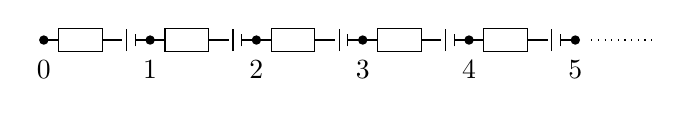
\begin{tikzpicture}[x=1.35cm,y=1cm]
  \foreach \i in {0,...,5}{\fill (\i,0) circle (1.7pt) node[below=4pt] {\i};}
  \foreach \i in {0,...,4}{
    \draw (\i,0)--(\i+0.14,0);
    \draw (\i+0.14,-0.15) rectangle (\i+0.55,0.15);
    \draw (\i+0.55,0)--(\i+0.74,0);
    \draw (\i+0.78,-0.14)--(\i+0.78,0.14);
    \draw (\i+0.86,-0.08)--(\i+0.86,0.08);
    \draw (\i+0.86,0)--(\i+1,0);
  }
  \draw[dotted] (5.15,0)--(5.75,0);
\end{tikzpicture}
\caption{线状电路“网络”}
\label{fig:line-network}
\end{figure}

我们注意到，此时的导纳矩阵十分特别：只有对角元和次对角元非零。我们将这样的矩阵称为三对角（tri-diagonal）矩阵。如果将 Gauß 消元法应用于该矩阵：首先消去第一列自第二行开始的非零元，而这样的非零元仅有一个，而在消去的过程中，第一行又只有两个非零元，做减除的时候计算消耗也是 $O(1)$ 的。随后消去第二列自第三行起的非零元，同样也只有一个。如此继续直至最后一行，我们可以仅以 $O(n)$ 的时间消耗完成三对角矩阵的求解，实际上，这个时间消耗和直接计算电路中流过的电流是一致的。

Gauß 消元法对于三对角矩阵的这个约化算法被称为追赶法（英文中称 tridiagonal matrix algorithm 或 Thomas algorithm）。记三对角矩阵的左次对角元为 $a_i$、对角元为 $b_i$、右次对角元为 $c_i$，右端向量的元素为 $d_i$，则追赶法的伪代码如下。

\begin{algorithmBox}[算法 3.4\quad 追赶法]
\begin{lstlisting}[style=bellacode]
function Tridiagonal(a,b,c,d)
    d(1) = d(1)/b(1)
    for i = 2, n
        c(i-1) = c(i-1)/b(i-1)
        b(i) = b(i)-a(i)*c(i-1)
        d(i) = (d(i)-a(i)*d(i-1))/b(i)
    end

    x(n) = d(n)
    for i = n-1, 1
        x(i) = d(i) - c(i)*x(i+1)
    end
end
\end{lstlisting}
\end{algorithmBox}

值得注意的是，上述算法是针对一般的三对角矩阵，如果考虑我们刚才所讨论的实际问题中的对称三对角矩阵，算法还可以进一步简化。

注意，直接将 Gauß 消元法不做修改应用于三对角矩阵时，计算复杂度不会下降——计算机计算 $0.0\times1.0$ 并不比计算 $1453.529\times1926.817$ 来得快。当计算中包含大量零元时，你必须明确告诉计算机哪些计算不需要进行。

更一般地，若一个矩阵 $A$ 满足对于任意 $|i-j|>k$ 都有 $(A)_{ij}=0$，我们将其称为带宽为 $2k+1$ 的带状矩阵（band matrix）。$k=0$ 对应于对角矩阵，而 $k=1$ 对应于三对角矩阵。容易检验，Gauß 消元法对于一般的带状矩阵都能做约化，其时间复杂度为 $O(nk^2)$。

我们同样可以从电路网络中找到带状矩阵的实际物理对应。

\begin{exerciseBox}[练习 3.1]
试证明，如图 3.2 所示的 $k$ 层带状电路的导纳矩阵可以写作带宽为 $2k+1$ 的带状矩阵，并据此说明，若将图 3.1 中的电路首尾相连，得到的导纳矩阵可以写成一个带宽为 5 的带状矩阵。
\end{exerciseBox}

\begin{figure}[htbp]
\centering
\begin{tikzpicture}[x=1.55cm,y=1.0cm,>=Stealth,font=\small]
  \foreach \x in {0,1,2,3,4}{
    \foreach \y in {0,1,2}{\fill (\x,\y) circle (1.5pt);}
  }
  \foreach \x in {0,...,4}{\draw (\x,0)--(\x,2);}
  \foreach \y in {0,1,2}{\draw (0,\y)--(4.35,\y);}
  \node[below left] at (0,0){0};
  \node[below] at (1,0){$k$};
  \node[below] at (2,0){$2k$};
  \node[below] at (3,0){$3k$};
  \node[below] at (4,0){$4k$};
  \node[left] at (0,1){2};
  \node[above left] at (0,2){$k-1$};
  \node at (1,0.45){$k+1$};
  \node at (2,0.45){$2k+1$};
  \node at (3,0.45){$3k+1$};
  \node at (4,0.45){$4k+1$};
  \node at (1,1.45){$k+2$};
  \node at (2,1.45){$2k+2$};
  \node at (3,1.45){$3k+2$};
  \node at (4,1.45){$4k+2$};
  \node[above] at (1,2){$2k-1$};
  \node[above] at (2,2){$3k-1$};
  \node[above] at (3,2){$4k-1$};
  \node[above] at (4,2){$5k-1$};
  \node at (0.5,1.5){$\cdots$};
  \node at (1.5,1.5){$\cdots$};
  \node at (2.5,1.5){$\cdots$};
  \node at (3.5,1.5){$\cdots$};
  \node at (4.28,1.5){$\cdots$};
\end{tikzpicture}
\caption{带状电路网络}
\label{fig:band-network}
\end{figure}

\section{暂态过程：二次型最优化与线性方程组的迭代解法}

我们回过头来考察上一节所提出的电路问题。它是否存在“物理”的解法呢？换句话说，我们能否从某个不满足方程
\begin{equation}
G\bm U=\bm J
\tag{3.2.1}
\end{equation}
的电压分布 $\bm U$ 出发，通过一些物理上的演化，让它最终满足方程呢？

答案是肯定的。假设电路中的每一个节点都各自通过一个电容接地\footnote{实际电路中真的存在类似的分布电容，以及分布电感和互感。}，然后给定一个初态电压分布 $\bm U(t=0)$。经过一系列的暂态过程后，各个电容上的电量不再变化，那么此时若切断全部的电容，系统的状态应当不变。换言之，我们将一个纯电阻网络的恒定电路问题转换成了一个 RC 暂态电路的末态问题。数学上，我们很容易给出微分方程
\begin{equation}
C\frac{d}{dt}\bm U(t)=\bm J-G\bm U(t),
\tag{3.2.2}
\end{equation}
它的解为
\begin{equation}
\bm U(t)=G^{-1}\bm J+e^{-tC^{-1}G}\left[\bm U(0)-G^{-1}\bm J\right],
\tag{3.2.3}
\end{equation}
其中电容矩阵 $C=\operatorname{diag}(C_1,C_2,\ldots,C_n)$ 给出了与各节点相连的电容。只要矩阵 $G$ 是正定的，当 $t\to\infty$ 时指数项趋近于零，微分方程组确实给出了线性代数方程组的解。

关于 $G$ 的正定性可以做如下证明。考虑内积
\begin{equation}
\begin{aligned}
\bm U^{\mathrm T}G\bm U
&=\sum_i\sum_{j\ne i}U_i g_{ij}(U_i-U_j)\\
&=\frac12\sum_{i,j}\left[U_i g_{ij}(U_i-U_j)+U_j g_{ji}(U_j-U_i)\right]\\
&=\frac12\sum_{i,j}g_{ij}(U_i-U_j)^2\\
&\ge0.
\end{aligned}
\tag{3.2.4}
\end{equation}
\jiaokan{原文式 (3.2.4) 第一行只写了 $\sum_{j\ne i}$，遗漏了对节点指标 $i$ 的求和。由 $\bm U^{\mathrm T}G\bm U$ 的矩阵乘法展开应为 $\sum_i\sum_{j\ne i}$；本版补入外层求和。}
在网络连通的前提下，当且仅当全部电势 $U_i$ 均相等时为零。进一步，删去第 $k$ 行和第 $k$ 列相当于将 $U_k$ 取作零，此时更是仅当余下电势均为零时二次型才为零。那么，我们便证明了删减后的导纳矩阵 $G$ 是对称正定的。

直观上想，求解微分方程组应当要比求解线性代数方程组更加困难，但这并不一定。我们对 (3.2.2) 式采用前向 Euler 法：
\begin{equation}
\bm U_{n+1}=\bm U_n+C^{-1}[\bm J-G\bm U_n]\Delta t.
\tag{3.2.5}
\end{equation}
可以看到计算过程中只涉及了矩阵向量乘法，如果矩阵 $G$ 是极端稀疏的，则乘法计算非常快。此外我们的目标是得到 $U(t)$ 在 $t\to\infty$ 时刻的值，并不要求精确计算其中间过程，从而时间步长 $\Delta t$ 也可以取得尽量大。那么综合看来，(3.2.5) 式这种一步步迭代的算法的效率不一定会比直接 Gauß 消元差。这也是本节的主题：线性代数方程组的迭代解法。

\subsection{Jacobi 迭代和 Gauß--Seidel 迭代}

对于更一般的问题
\begin{equation}
A\bm x=\bm b,
\tag{3.2.6}
\end{equation}
只要矩阵 $A$ 正定，原则上我们都可以通过计算迭代式
\begin{equation}
\bm x_{n+1}=\bm x_n+B[\bm b-A\bm x_n]\Delta t
\tag{3.2.7}
\end{equation}



我们令矩阵按照对角元、下三角元和上三角元做分解：
\begin{equation}
A=D+L+U.
\tag{3.2.8}
\end{equation}
那么，迭代格式
\begin{equation}
\bm y^{(k+1)}=D^{-1}\left[\bm b-(L+U)\bm y^{(k)}\right]
\tag{3.2.9}
\end{equation}
被称为 Jacobi 迭代，这相当于取 $B$ 为 $A$ 对角元的逆，并令 $\Delta t=1$。当矩阵 $A$ 的全部对角元的绝对值大于等于其所在行非对角元绝对值之和，即主对角占优时，算法是一定收敛的。读者可以自行检验电路网络问题满足这个条件。Jacobi 迭代的伪代码如下。

\begin{algorithmBox}[算法 3.5\quad Jacobi 迭代]
\begin{lstlisting}[style=bellacode]
function JacobiIteration(n,A,y,b)
    do i = 1, n
        ny(i) = b(i)
        do j = 1, n
            if(j=i) cycle
            ny(i) = ny(i) - A(i,j)*y(j)
        end
        ny(i) = ny(i)/A(i,i)
    end
    return ny
end
\end{lstlisting}
\end{algorithmBox}

注意函数 \texttt{JacobiIteration} 仅给出了单步迭代的步骤，完整求解问题还需要加入收敛判据并重复调用。

Jacobi 迭代的一个推广形式是 Gauß--Seidel 迭代：
\begin{equation}
\bm y^{(k+1)}=(D+L)^{-1}\left(-U\bm y^{(k)}+\bm b\right).
\tag{3.2.10}
\end{equation}
实践上，我们将其写为
\[
\bm y^{(k+1)}=D^{-1}\left(\bm b-U\bm y^{(k)}-L\bm y^{(k+1)}\right).
\]
注意上式与 (3.2.9) 式的区别，利用上三角元和下三角元在做矩阵乘法时的特殊性，这个迭代格式相当于在逐行计算 Jacobi 迭代的矩阵乘法过程中，在等式右端替换了那些已经完成计算的元素。其伪代码如下。

\begin{algorithmBox}[算法 3.6\quad Gauß--Seidel 迭代]
\begin{lstlisting}[style=bellacode]
function GaussSeidel(n,A,y,b)
    do i = 1, n
        y(i) = b(i)
        do j = 1, n
            if(j>=i) cycle
            y(i) = y(i) - A(i,j)*y(j)
        end
        y(i) = y(i)/A(i,i)
    end
    return y
end
\end{lstlisting}
\end{algorithmBox}
\jiaokan{原算法第 5 行写作 \texttt{if(j>i) cycle}，从而 $j=i$ 时仍会执行第 6 行，用尚未除以 $A(i,i)$ 的当前 $y(i)$ 自身作减法，和式 (3.2.10) 不一致。Gauß--Seidel 的逐行更新在此只应累加 $j<i$ 的下三角项，故本版将条件改为 \texttt{if(j>=i) cycle}。}

Gauß--Seidel 迭代的计算量与 Jacobi 迭代相当，但是存储空间省了一半。通常而言，如果矩阵 $A$ 对 Jacobi 迭代和 Gauß--Seidel 迭代均收敛，那么 Gauß--Seidel 迭代的收敛率约为前者的两倍。

这类直接利用方程构造迭代关系的算法有很多变种，如松弛迭代、超松弛迭代等等，其收敛性和收敛速度都难以事先判断，主要由迭代矩阵的谱半径决定，感兴趣的读者可参考其他文献，我们在此不做更多介绍。

\subsection{向量范数与矩阵范数}

上文中略过了迭代算法所必需的终止条件，即收敛判据。此处用于迭代的是向量，迭代收敛可能的一个判据自然是相邻两步向量之差 $\bm y^{(k+1)}-\bm y^{(k)}$ 充分接近于零向量。为此，我们需要有一个函数，用以描述某个向量与零向量的接近程度，而这个函数便是向量范数。

设对于任意向量 $\bm x\in\mathbb R^n$，都有唯一实数 $\|\bm x\|\in\mathbb R$ 与其对应，且该映射满足：
\begin{enumerate}
\item 正定性，$\|\bm x\|\ge0$，等号仅当 $\bm x=0$ 时成立；
\item 齐次性，对于任意 $a\in\mathbb R$，有 $\|a\bm x\|=|a|\|\bm x\|$；
\item 三角不等式，$\|\bm x+\bm y\|\le\|\bm x\|+\|\bm y\|$，其中当 $\bm y=a\bm x\,(a\in\mathbb R)$ 时等号成立。
\end{enumerate}
那么我们称 $\|\bm x\|$ 为 $\bm x$ 的范数。

满足上述三个条件的范数有许多种，例如 $p$-范数：
\begin{equation}
\|\bm x\|_p=\left(\sum_{i=1}^{n}|x_i|^p\right)^{1/p},\qquad p\ge1.
\tag{3.2.11}
\end{equation}
$p$ 分别取 $1,2$ 和 $\infty$ 时对应着三种常用的向量范数，即
\begin{enumerate}
\item 1-范数 $\|\bm x\|_1=|x_1|+|x_2|+\cdots+|x_n|$；
\item 2-范数／欧氏范数 $\|\bm x\|_2=\sqrt{x_1^2+x_2^2+\cdots+x_n^2}$；
\item $\infty$-范数 $\|\bm x\|_\infty=\max_i|x_i|$。
\end{enumerate}
此外，对于对称正定矩阵 $S$，我们也可以根据其二次型来定义范数：
\begin{equation}
\|\bm x\|_S\equiv\sqrt{\bm x^{\mathrm T}S\bm x}.
\tag{3.2.12}
\end{equation}

在有了向量范数概念后，我们便可以选择一个合适且方便计算的范数定义，来给出迭代算法的收敛判据了。可以证明，对于向量序列 $\{\bm x_0,\bm x_1,\bm x_2,\ldots\}$，如果它在某个范数定义下收敛于 $\bm x^*$，即
\begin{equation}
\lim_{k\to\infty}\|\bm x_k-\bm x^*\|=0,
\tag{3.2.13}
\end{equation}
那么它在任意范数定义下都收敛。

除了向量范数，我们同样可以对于矩阵定义范数。此时除去之前的三个条件外，还会引入一个额外的相容性条件：
\begin{enumerate}
\item 正定性，$\|A\|\ge0$，等号仅当 $A=0$ 时成立；
\item 齐次性，对于任意 $a\in\mathbb R$，有 $\|aA\|=|a|\|A\|$；
\item 三角不等式，$\|A+B\|\le\|A\|+\|B\|$；
\item 相容性，$\|AB\|\le\|A\|\|B\|$。
\end{enumerate}
如果预先定义了向量范数，我们通常也要求矩阵范数与其相容：
\begin{equation}
\|A\bm x\|\le\|A\|\|\bm x\|.
\tag{3.2.14}
\end{equation}
与三种 $p$-范数相容的矩阵范数分别为：
\begin{enumerate}
\item 列范数 $\|A\|_1=\max_j\sum_i|a_{ij}|$；
\item 谱范数 $\|A\|_2=\max_i\sqrt{\lambda_i}$，这里 $\lambda_i$ 为矩阵 $A^{\mathrm T}A$ 的本征值；
\item 行范数 $\|A\|_\infty=\max_i\sum_j|a_{ij}|$。
\end{enumerate}
此外，Frobenius 范数 $\|A\|_{\mathrm F}=\sqrt{\operatorname{trace}(A^{\mathrm T}A)}$ 同样与向量的 2-范数相容。在后续章节中我们也将看到矩阵范数的一些应用。

前面讨论过，一个实际问题转化为数学问题时，初始数据往往会有观测误差和舍入误差，亦即扰动，从而使得最终计算结果产生误差。向量的误差可以用向量的范数表示：设 $\bm x^*$ 是 $\bm x$ 的近似向量，$\|\bm x-\bm x^*\|$、$\|\bm x-\bm x^*\|/\|\bm x^*\|$ 分别称为 $\bm x^*$ 的关于范数 $\|\bullet\|$ 的绝对误差与相对误差。矩阵的误差可以用矩阵算子范数表示：设 $A^*$ 是 $A$ 的近似矩阵，$\|A-A^*\|$、$\|A-A^*\|/\|A^*\|$ 分别称为 $A^*$ 的关于范数 $\|\bullet\|$ 的绝对误差与相对误差。根据范数的等价性，用何种向量范数都是合理的，取决于实际过程中是否容易计算。对理论分析，谱范数是非常有效的，但是在计算上，行范数和列范数更加方便。

比较下面两个方程组：
\[
\left\{\begin{aligned}
x_1+x_2&=2,\\
x_1+1.00001x_2&=2
\end{aligned}\right.
\quad\Longrightarrow\quad
\left\{\begin{aligned}x_1&=2,\\x_2&=0,
\end{aligned}\right.
\]
\[
\left\{\begin{aligned}
x_1+x_2&=2,\\
x_1+1.00001x_2&=2.00001
\end{aligned}\right.
\quad\Longrightarrow\quad
\left\{\begin{aligned}x_1&=1,\\x_2&=1.
\end{aligned}\right.
\]
显然，二者只是在右端项有很小的差别，最大相对误差仅为 $\frac12\times10^{-5}$，但是它们的解截然不同，解的分量的相对误差至少为 $\frac12$。对于以上系数矩阵的方程组，输入数据的误差对解的结果影响巨大。由此，我们给出线性方程组的性态的定义。

\textbf{定义 3.1}\quad 如果矩阵 $A$ 或者右端项 $\bm b$ 的微小变化，可以引起方程组 $A\bm x=\bm b$ 解的巨大变化，则称此方程组为“病态”方程组，矩阵 $A$ 相对于该方程组而言称为病态矩阵，否则称方程组为“良态”方程组，$A$ 称为良态矩阵。

注意，矩阵的病态性质是矩阵本身的特性。

为了定量刻画方程组 $A\bm x=\bm b$ 的病态程度，可分别对方程组的系数矩阵和右端项有扰动时的两种情形进行讨论。

设 $\bm b$ 有扰动 $\delta\bm b$，相应的解 $\bm x$ 的扰动记为 $\delta\bm x$，即 $A(\bm x+\delta\bm x)=\bm b+\delta\bm b$。因此
\[
A\bm x=\bm b\quad\Rightarrow\quad A\delta\bm x=\delta\bm b
\quad\Rightarrow\quad \delta\bm x=A^{-1}\delta\bm b.
\]
两边取范数得到 $\|\delta\bm x\|=\|A^{-1}\delta\bm b\|\le\|A^{-1}\|\|\delta\bm b\|$。又因为 $\|A\bm x\|\le\|A\|\|\bm x\|$，有
\[
\|\bm x\|\ge\frac{\|A\bm x\|}{\|A\|}=\frac{\|\bm b\|}{\|A\|},
\]
故
\[
\frac{\|\delta\bm x\|}{\|\bm x\|}
\le
\frac{\|A^{-1}\|\|\delta\bm b\|}{\|\bm b\|/\|A\|}
=
\frac{\|A\|\|A^{-1}\|\|\delta\bm b\|}{\|\bm b\|}.
\]
上式表明，当右端项有扰动时，解的相对误差不超过右端项的相对误差的 $\|A\|\|A^{-1}\|$ 倍。

如果右端项没有扰动，而是系数矩阵 $A$ 有扰动 $\delta A$，相应的解的扰动仍然记为 $\delta\bm x$，则
\[
(A+\delta A)(\bm x+\delta\bm x)=\bm b
\quad\Rightarrow\quad
A\delta\bm x+\delta A(\bm x+\delta\bm x)=0
\]
\[
\Rightarrow\quad
\|\delta\bm x\|=\|A^{-1}\delta A(\bm x+\delta\bm x)\|
\le\|A^{-1}\|\|\delta A\|(\|\bm x\|+\|\delta\bm x\|).
\]
如果 $\delta A$ 充分小，使得 $\|A^{-1}\|\|\delta A\|<1$，则由上式得
\[
\|\delta\bm x\|\left(1-\|A^{-1}\|\|\delta A\|\right)
\le\|A^{-1}\|\|\delta A\|\|\bm x\|,
\]
故
\[
\frac{\|\delta\bm x\|}{\|\bm x\|}
\le
\frac{\|A^{-1}\|\|\delta A\|}{1-\|A^{-1}\|\|\delta A\|}
=
\frac{\|A\|\|A^{-1}\|\,\dfrac{\|\delta A\|}{\|A\|}}
{1-\|A\|\|A^{-1}\|\,\dfrac{\|\delta A\|}{\|A\|}}.
\]
此式表明，当系数矩阵有扰动时，解的扰动仍然与 $\|A\|\|A^{-1}\|$ 有关。$\|A\|\|A^{-1}\|$ 越大，通常所导致的解的扰动也越大。

综上分析可知，$\|A\|\|A^{-1}\|$ 实际上刻画了解对原始数据变化的敏感程度，即刻画了方程组的“病态”程度。

\textbf{定义 3.2}\quad 设 $A$ 为非奇异矩阵，称数
\[
\operatorname{cond}(A)_\nu\equiv\|A\|_\nu\|A^{-1}\|_\nu,\qquad \nu=1,2,\infty,
\]
为矩阵的条件数（condition number）。

常用的条件数有：
\begin{enumerate}
\item $\operatorname{cond}(A)_\infty=\|A^{-1}\|_\infty\|A\|_\infty$；
\item $A$ 的谱条件数
\[
\operatorname{cond}(A)_2=\|A^{-1}\|_2\|A\|_2
=\sqrt{\frac{\lambda_{\max}(A^{\mathrm T}A)}{\lambda_{\min}(A^{\mathrm T}A)}}.
\]
当 $A$ 为对称矩阵时，$\operatorname{cond}(A)_2=|\lambda_1|/|\lambda_n|$，其中 $\lambda_1$ 和 $\lambda_n$ 为矩阵 $A$ 的绝对值最大和绝对值最小的本征值。
\end{enumerate}

矩阵的条件数有如下性质：
\begin{enumerate}
\item 对任意非奇异矩阵 $A$，都有
\begin{equation}
\operatorname{cond}(A)_\nu\ge1.
\tag{3.2.15}
\end{equation}
这是因为
\[
\operatorname{cond}(A)_\nu=\|A^{-1}\|_\nu\|A\|_\nu
\ge\|A^{-1}A\|_\nu=\|I\|=1.
\]
\item 设 $A$ 为非奇异矩阵且 $c$ 为不为零的常数，则 $\operatorname{cond}(cA)_\nu=\operatorname{cond}(A)_\nu$。
\item 如果 $A$ 为正交矩阵，则 $\operatorname{cond}(A)_2=1$。
\item 如果 $A$ 为非奇异矩阵，$R$ 为正交矩阵，对谱条件数有
\[
\operatorname{cond}(RA)_2=\operatorname{cond}(AR)_2=\operatorname{cond}(A)_2.
\]
\end{enumerate}

针对矩阵条件数，我们来看一个例子。对 Hilbert 矩阵
\[
H_n=\begin{pmatrix}
1&\dfrac12&\cdots&\dfrac1n\\
\dfrac12&\dfrac13&\cdots&\dfrac1{n+1}\\
\vdots&\vdots&\ddots&\vdots\\
\dfrac1n&\dfrac1{n+1}&\cdots&\dfrac1{2n-1}
\end{pmatrix},
\]
试计算 $n=3$ 时的条件数：
\[
H_3=\begin{pmatrix}
1&\frac12&\frac13\\
\frac12&\frac13&\frac14\\
\frac13&\frac14&\frac15
\end{pmatrix},\qquad
H_3^{-1}=\begin{pmatrix}
9&-36&30\\
-36&192&-180\\
30&-180&180
\end{pmatrix}.
\]
通过计算可得
\[
\operatorname{cond}(H_3)_\infty=\|H_3\|_\infty\|H_3^{-1}\|_\infty
=\frac{11}{6}\times408=748.
\]
同理可计算得到
\[
\operatorname{cond}(H_6)_\infty=2.9\times10^6.
\]
事实上，Hilbert 矩阵是一种著名的病态矩阵，阶数 $n$ 越大，其条件数越大、病态性越严重。考虑一个例子：
\[
H_3\begin{pmatrix}x_1\\x_2\\x_3\end{pmatrix}
=
\begin{pmatrix}\frac{11}{6}\\\frac{13}{12}\\\frac{47}{60}\end{pmatrix}
\quad\Rightarrow\quad
\left\{\begin{aligned}x_1&=1,\\x_2&=1,\\x_3&=1.\end{aligned}\right.
\]
假设 $H_3$ 和 $\bm b$ 有微小的误差，$(H_3+\delta H_3)(\bm x+\delta\bm x)=\bm b+\delta\bm b$。这里，我们取 3 位有效数字，则
\[
\begin{pmatrix}
1.00&0.500&0.333\\
0.500&0.333&0.250\\
0.333&0.250&0.200
\end{pmatrix}
\begin{pmatrix}x_1+\delta x_1\\x_2+\delta x_2\\x_3+\delta x_3\end{pmatrix}
=
\begin{pmatrix}1.83\\1.08\\0.783\end{pmatrix},
\]
其解为 $\bm x+\delta\bm x=(1.0895,0.4880,1.491)^{\mathrm T}$，故 $\delta\bm x=(0.0895,-0.5120,0.4910)^{\mathrm T}$。由此，可以计算得到
\[
\frac{\|\delta H_3\|_\infty}{\|H_3\|_\infty}\approx0.18\times10^{-3}<0.02\%,\qquad
\frac{\|\delta\bm b\|_\infty}{\|\bm b\|_\infty}\approx0.182\%,\qquad
\frac{\|\delta\bm x\|_\infty}{\|\bm x\|_\infty}\approx\frac{0.5120}{1}=51.2\%.
\]
这表明，矩阵和右端项相对误差不超过 $0.2\%$，可是引起解的相对误差超过了 $50\%$！

计算条件数需要求矩阵的逆矩阵，因而代价比较大。根据数值经验，在下列情况下，方程组常常是病态的：
\begin{enumerate}
\item 在使用主元消去法时出现小主元；
\item $A$ 的最大特征值和最小特征值绝对值之比很大；
\item 系数矩阵中有行或列近似线性相关，或系数行列式的值近似为零，但这不是绝对的，例如当 $A=\epsilon I$，$\epsilon$ 是很小的数时，有 $\det(A)=\epsilon^n\approx0$，但是 $\operatorname{cond}(A)=\operatorname{cond}(I)=1$，方程组是良态的；
\item 系数矩阵 $A$ 元素间数量级相差很大，并且没有一定的规则。
\end{enumerate}

\subsection{最速下降法}

我们希望找到一种收敛性更好的迭代算法。暂时先假设矩阵 $A$ 对称正定，那么可以考察如下形式的极小值问题：
\begin{equation}
\min_{\bm x} f(\bm x)\equiv\frac12\bm x^{\mathrm T}A\bm x-\bm b^{\mathrm T}\bm x
=\frac12(\bm x-A^{-1}\bm b)^{\mathrm T}A(\bm x-A^{-1}\bm b)-\frac12\bm b^{\mathrm T}A^{-1}\bm b.
\tag{3.2.16}
\end{equation}
由于 $A$ 正定，函数存在最小值，当 $\bm x$ 取原线性方程组的解时达到。我们将一个线性方程组的求解转换成了一个等价的函数极小值问题。注意到，如果回到电路网络问题，函数 $f(\bm x)$ 实际上给出了电路中全部电阻元件的功率消耗（只相差一个常数）。在物理上，这个等价转换是广义变分原理在电路问题上的特例：闭合电路中的真实电势分布使得功率消耗取极小值。

我们在第 2.5 节中讨论过一维函数的最优化问题，大致思路是从某一个点或几个点出发，利用这些点附近的信息在一维区间选取下一个点，不断搜索。而现在到了多自由度的问题，从一个点出发不仅需要知道往前走多远，还得知道往什么方向走。最直接的想法是寻找在该点处函数值下降最快的方向，即负梯度方向。考虑我们有初始猜测值 $\bm x_0$，此处的负梯度为
\begin{equation}
-\nabla f(\bm x_0)=\bm b-A\bm x_0,
\tag{3.2.17}
\end{equation}
记作 $\bm r_0$。随后就是考虑该走多远。计算
\begin{equation}
\begin{aligned}
f(\bm x_0+\alpha\bm r_0)
&=\frac{\alpha^2}{2}\bm r_0^{\mathrm T}A\bm r_0
+\alpha(A\bm x_0-\bm b)^{\mathrm T}\bm r_0\\
&\quad+\frac12\bm x_0^{\mathrm T}A\bm x_0-\bm b^{\mathrm T}\bm x_0.
\end{aligned}
\tag{3.2.18}
\end{equation}
它是关于参数 $\alpha$ 的二次函数，其极小值点容易算得：
\begin{equation}
\alpha=\frac{\bm r_0^{\mathrm T}\bm r_0}{\bm r_0^{\mathrm T}A\bm r_0}.
\tag{3.2.19}
\end{equation}
得到下一个点 $\bm x_1=\bm x_0+\alpha\bm r_0$。依次循环往复，就能逐步逼近问题的解了。这个思路被称作最速下降法（steepest descent method）。注意到，在理论上函数极值点处梯度为零，$\bm r_0^{\mathrm T}\bm r_0=0$，我们可以依此作为收敛判据。伪代码如下。

\begin{algorithmBox}[算法 3.7\quad 最速下降法（二次型）]
\begin{lstlisting}[style=bellacode]
function SteepestDescent(A,b,x,eps)
    r = b - A.x
    resi = r.r
    do while(resi>eps)
        q = A.r
        alpha = resi/(r.q)
        x = x + alpha * r
        r = r - alpha * q
        resi = r.r
    end
    return x
end
\end{lstlisting}
\end{algorithmBox}

这里下角点“.”代表将前一个数组的最后一个指标和后一个数组的第一个指标缩并，相应于矩阵乘法。注意我们引入了额外的辅助变量 $\bm q=A\bm r$ 以节省一次矩阵乘法的计算。$\bm r^{\mathrm T}\bm q$ 出现在了分母上作为除数，由于我们假定了矩阵 $A$ 正定，可知其必定大于零。

整个计算中只出现了矩阵和向量的乘法，单次迭代的时间消耗是 $O(n^2)$。对于非零元素数目 $N\ll n^2$ 的稀疏矩阵，矩阵乘法的消耗更是降低至 $O(N)$。那么，只要迭代法能够在 $O(n)$ 步内给出一个精度可以接受的结果，这个迭代解法就不比直接用 Gauß 消元法差。而对于充分稀疏的矩阵，迭代算法更是远优于上一节中的直接解法。

那么梯度下降法的收敛速度如何呢？我们可以考察相邻两步待优化函数值与最优值之差 $f(\bm x_k)-f(\bm x^*)$ 的比值。简单的计算给出
\begin{equation}
\frac{f(\bm x_{k+1})-f(\bm x^*)}{f(\bm x_k)-f(\bm x^*)}
=1-\frac{(\bm r_k^{\mathrm T}\bm r_k)^2}{(\bm r_k^{\mathrm T}A^{-1}\bm r_k)(\bm r_k^{\mathrm T}A\bm r_k)}.
\tag{3.2.20}
\end{equation}
令 $\bm u=A^{-1/2}\bm r$，可以发现上式实际上就等于向量 $\bm u$ 与 $A\bm u$ 夹角正弦的平方值。正弦平方的下界是零，而上界则在向量 $\bm u$ 与 $A\bm u$ 的方向偏离最远的时候取到。显然，此时 $\bm u$ 肯定位于矩阵 $A$ 最大本征值 $\lambda_{\max}$ 和最小本征值 $\lambda_{\min}$ 所分别对应的两个本征向量构成的子空间内。进一步放缩不等式可以求得
\begin{equation}
\frac{f(\bm x_{k+1})-f(\bm x^*)}{f(\bm x_k)-f(\bm x^*)}
\le\left(\frac{\kappa-1}{\kappa+1}\right)^2<1.
\tag{3.2.21}
\end{equation}
此处我们引入了记号 $\kappa=|\lambda_{\max}/\lambda_{\min}|\ge1$，也就是对称矩阵的谱条件数。上述讨论中，$\bm u$ 与 $A\bm u$ 的关系如图 3.3 所示。

\begin{figure}[htbp]
\centering
\begin{tikzpicture}[x=1.3cm,y=1.3cm,>=Stealth]
  \draw[->] (0,0)--(4.3,0);
  \draw[->] (0,0)--(0,3.1);
  \draw[->,thick] (0,0)--(1.2,2.35) node[above right] {$\bm u$};
  \draw[->,thick] (0,0)--(3.45,1.62) node[above right] {$A\bm u$};
  \draw[dashed] (1.2,0)--(1.2,2.35);
  \draw[dashed] (0,2.35)--(1.2,2.35);
  \draw[dashed] (3.45,0)--(3.45,1.62);
  \draw[dashed] (0,1.62)--(3.45,1.62);
  \node[below] at (1.2,0) {$u_1$};
  \node[left] at (0,2.35) {$u_2$};
  \node[below] at (3.45,0) {$\lambda_1u_1$};
  \node[left] at (0,1.62) {$\lambda_2u_2$};
\end{tikzpicture}
\caption{向量 $\bm u$ 与 $A\bm u$ 的示意图，图中相应于 $\kappa=|\lambda_1/\lambda_2|=5$ 的情形。当 $(u_2/u_1)^2=\kappa$ 时，这两个向量夹角正弦最大}
\label{fig:u-Au}
\end{figure}

这种相邻两步误差之比为常数的形式我们之前见过，为线性收敛，收敛率上界为 $[(\kappa-1)/(\kappa+1)]^2$。当 $\kappa\gg1$ 时，算法会几乎退化为弱线性收敛，而若 $\kappa=1$，一步就能收敛，此时矩阵为单位阵简单乘上一个常数。

再次强调，条件数是一个非常重要的概念，它将在本书随后的章节以及数值实践中与大家时刻相伴。这里我们看到大条件数矩阵很难用迭代法处理，实际上在直接法数值求解线性方程组的过程中，大条件数的矩阵也会造成舍入误差被快速放大，导致得到的“精确解”的精度难以接受。由此，我们将大条件数的矩阵及其对应的问题称作刚性（stiffness），甚至是病态的（ill-conditioned）。

(3.2.21) 式给出的是收敛率的一个上界。但可以证明，只要猜测解中包含了本征值 $\lambda_{\max}$ 和 $\lambda_{\min}$ 所分别对应的两个本征向量的分量，在 $n\to\infty$ 时，相邻两步误差之比一定会收敛到这个上界，并且 $\bm r_k$ 也会落到这两个本征向量所张成的子空间中。这可就让人头疼了：明明近乎在一个二维平面内找极小值，为什么就不能迅速收敛到真实解呢？这便引出了下一小节的主题——共轭梯度法。

\subsection{共轭梯度法}

我们重新来考察 (3.2.16) 式给出的最优化问题。在给出一个初始猜测解 $\bm x_0$ 后，第一步 $\bm p_0$ 依旧取在函数梯度方向上：
\begin{equation}
\left\{\begin{aligned}
\bm r_0&=\bm b-A\bm x_0,\\
\bm p_0&=\bm r_0,\\
\alpha_0&=\frac{\bm r_0^{\mathrm T}\bm p_0}{\bm p_0^{\mathrm T}A\bm p_0},\\
\bm x_1&=\bm x_0+\alpha_0\bm p_0,\\
\bm r_1&=\bm r_0-\alpha_0A\bm p_0.
\end{aligned}\right.
\tag{3.2.22}
\end{equation}
引入记号 $\bm p$ 是为了后续叙述方便，读者可以检验上式中 $\alpha$ 的选取当搜索方向不在函数梯度的方向上时也成立。此时我们获得了两个向量：上一步的搜索方向 $\bm p_0$ 和这一步的残差 $\bm r_1$。容易检验它们是正交的，$\bm p_0^{\mathrm T}\bm r_1=0$。在第二步，我们就不限定搜索方向在 $\bm r_1$ 了，而是在子空间 $\operatorname{span}\{\bm p_0,\bm r_1\}$ 中寻找函数极小值，这样就提前避免了最速下降法最后面临的困难。具体来说，考察函数
\begin{equation}
\begin{aligned}
f(\bm x_1+\xi\bm r_1+\eta\bm p_0)
&=\frac12(\xi\bm r_1+\eta\bm p_0)^{\mathrm T}A(\xi\bm r_1+\eta\bm p_0)\\
&\quad +(A\bm x_1-\bm b)^{\mathrm T}(\xi\bm r_1+\eta\bm p_0)
+\frac12\bm x_1^{\mathrm T}A\bm x_1-\bm b^{\mathrm T}\bm x_1.
\end{aligned}
\tag{3.2.23}
\end{equation}
它是关于 $\xi,\eta$ 的二元二次函数。对 $\eta$ 偏导数为零给出
\begin{equation}
(\xi\bm r_1+\eta\bm p_0)^{\mathrm T}A\bm p_0=\bm r_1^{\mathrm T}\bm p_0=0,
\tag{3.2.24}
\end{equation}
即新的搜索方向 $\alpha_1\bm p_1=\xi\bm r_1+\eta\bm p_0$ 与 $A\bm p_0$ 正交。我们可以将 $\bm p_1$ 取作
\begin{equation}
\bm p_1=\bm r_1+\beta_0\bm p_0,
\tag{3.2.25}
\end{equation}
其中 $\beta_0=-\bm p_0^{\mathrm T}A\bm r_1/(\bm p_0^{\mathrm T}A\bm p_0)$。这相当于用 $\bm p_0$ 扣除掉 $\bm r_1$ 中与 $A\bm p_0$ 平行的分量。相应的步长 $\alpha_1$ 可以参照之前的一维搜索给出：
\begin{equation}
\left\{\begin{aligned}
\alpha_1&=\frac{\bm r_1^{\mathrm T}\bm p_1}{\bm p_1^{\mathrm T}A\bm p_1},\\
\bm r_2&=\bm r_1-\alpha_1A\bm p_1.
\end{aligned}\right.
\tag{3.2.26}
\end{equation}
这种形式的搜索依旧保证了正交关系 $\bm p_1^{\mathrm T}\bm r_2=0$。

到了这一步，我们就可以放心大胆地依次迭代下去了，迭代关系为
\begin{equation}
\bm p_k=\bm r_k+\beta_{k-1}\bm p_{k-1},\qquad
\beta_{k-1}=-\frac{\bm p_{k-1}^{\mathrm T}A\bm r_k}{\bm p_{k-1}^{\mathrm T}A\bm p_{k-1}},
\tag{3.2.27}
\end{equation}
\begin{equation}
\bm r_{k+1}=\bm r_k-\alpha_kA\bm p_k,\qquad
\alpha_k=\frac{\bm r_k^{\mathrm T}\bm p_k}{\bm p_k^{\mathrm T}A\bm p_k}.
\tag{3.2.28}
\end{equation}

在给出具体代码之前，我们仍要对计算过程做一定的化简。$\bm p_{k-1}^{\mathrm T}\bm r_k=0$ 与 (3.2.27) 式联立可以推出 $\bm r_k^{\mathrm T}\bm p_k=\bm r_k^{\mathrm T}\bm r_k$，从而可以简化 $\alpha_k$ 的计算。进一步有
\begin{equation}
\begin{aligned}
\bm r_k^{\mathrm T}\bm r_{k+1}
&=\bm r_k^{\mathrm T}\bm r_k-
\frac{\bm r_k^{\mathrm T}\bm r_k}{\bm p_k^{\mathrm T}A\bm p_k}\bm r_k^{\mathrm T}A\bm p_k\\
&=\frac{\bm r_k^{\mathrm T}\bm r_k}{\bm p_k^{\mathrm T}A\bm p_k}
(\bm p_k-\bm r_k)^{\mathrm T}A\bm p_k\\
&=0,
\end{aligned}
\tag{3.2.29}
\end{equation}
即相邻两步的残差正交。而另一方面
\begin{equation}
\begin{aligned}
\beta_{k-1}
&=-\frac{\bm p_{k-1}^{\mathrm T}A\bm r_k}{\bm p_{k-1}^{\mathrm T}A\bm p_{k-1}}\\
&=\frac{\alpha_{k-1}^{-1}(\bm r_k-\bm r_{k-1})^{\mathrm T}\bm r_k}{\bm p_{k-1}^{\mathrm T}A\bm p_{k-1}}\\
&=\frac{\bm r_k^{\mathrm T}\bm r_k}{\bm r_{k-1}^{\mathrm T}\bm r_{k-1}},
\end{aligned}
\tag{3.2.30}
\end{equation}
为相邻两步残差模方之比。这样，最后的伪代码如下。

\begin{algorithmBox}[算法 3.8\quad 共轭梯度法（二次型）]
\begin{lstlisting}[style=bellacode]
function ConjugateGradient(A,b,x,eps)
    r = b - A.x
    p = r
    oldResi = r.r
    do while(oldResi>eps)
        q = A.p
        alpha = oldResi/(p.q)
        x = x + alpha * p
        r = r - alpha * q
        newResi = r.r
        beta = newResi/oldResi
        p = r + beta * p
        oldResi = newResi
    end
    return x
end
\end{lstlisting}
\end{algorithmBox}

这个算法被称为共轭梯度法，其名字的含义相信读者通过上面讨论的各向量之间无穷无尽的正交关系已经看出端倪了。共轭梯度法每一步迭代仅需要一次矩阵向量乘法，与最速下降法的计算消耗相同，而如我们一开头所讨论的，其每一步都在一个二维平面内寻找极值，收敛速度上显著优于最速下降法。事实上，共轭梯度法原则上可以在 $n$ 次迭代内得到精确解！

我们来具体考察这个惊人的事实：在 (3.2.27) 式两端左乘 $A$，并代入 (3.2.28) 式消去 $\bm p$，我们得到
\begin{equation}
\bm r_{k+1}=-\alpha_kA\bm r_k+
\left(1+\beta_{k-1}\frac{\alpha_k}{\alpha_{k-1}}\right)\bm r_k
-\beta_{k-1}\frac{\alpha_k}{\alpha_{k-1}}\bm r_{k-1}.
\tag{3.2.31}
\end{equation}
之前我们已经证明了 $\bm r_k^{\mathrm T}\bm r_{k+1}=0$，而再压低一个指标，
\begin{equation}
\begin{aligned}
\bm r_{k-1}^{\mathrm T}\bm r_{k+1}
&=-\alpha_k\bm r_{k-1}^{\mathrm T}A\bm r_k
-\beta_{k-1}\frac{\alpha_k}{\alpha_{k-1}}\bm r_{k-1}^{\mathrm T}\bm r_{k-1}\\
&=\beta_{k-2}\frac{\alpha_k}{\alpha_{k-2}}\bm r_{k-2}^{\mathrm T}\bm r_k.
\end{aligned}
\tag{3.2.32}
\end{equation}
将上式反复用自身迭代，并利用 $\bm r_0^{\mathrm T}\bm r_2=0$ 这一事实，可以得到 $\bm r_k^{\mathrm T}\bm r_{k+2}=0$。以此类推，我们最终可以证明所有 $\bm r_k$ 都是相互正交的：
\begin{equation}
\bm r_i^{\mathrm T}\bm r_j=0,\qquad i\ne j.
\tag{3.2.33}
\end{equation}

现在我们得到了所需要的性质。在进行共轭梯度迭代的过程中，我们实际上构造了一个由向量组 $\{\bm r_0,A\bm r_0,A^2\bm r_0,\ldots,A^k\bm r_0\}$ 张成的子空间，称作 \rusname{Крылов} 子空间 $K_k(A,\bm r_0)$，并且找到了这个子空间中的一组正交基组 $\{\bm r_0,\bm r_1,\ldots,\bm r_k\}$。由 (3.2.31) 式可知，矩阵 $A$ 在这个基组下表现为一个三对角矩阵，而三对角矩阵可以通过追赶法简单求解。当迭代次数增加时，子空间维度逐步增大，而当维度等同于全空间维度 $n$ 时，得到的解就是问题的精确解。

当然上述的论述中还有一些缺漏的地方。比方说，如果初始残差 $\bm r_0$ 一开始位于矩阵 $A$ 某几个本征向量构成的子空间内，那么不管再怎么计算 $A^k\bm r_0$，其都不可能跑出这个不变子空间。但这其实是好事，因为我们的目的就是为了让最后的 $\bm r_k$ 变成零，而维度变小反而意味着收敛到精确解的迭代次数变少了。

虽然理论上讲共轭梯度法能够在有限步内给出精确解，但计算复杂度相比 Gauß 消元法并不占优，且由于在构造正交基组过程中舍入误差的放大，实践上它也很难真正给出一个精确解。因此实践上，人们通常还是将其看作一个迭代解法。标准的全局误差估计为
\begin{equation}
\frac{f(\bm x_k)-f(\bm x^*)}{f(\bm x_0)-f(\bm x^*)}
\le 4\left(\frac{\sqrt\kappa-1}{\sqrt\kappa+1}\right)^{2k}.
\tag{3.2.34}
\end{equation}
\jiaokan{原文将式 (3.2.34) 写成相邻两步函数误差之比 $[f(\bm x_{k+1})-f(\bm x^*)]/[f(\bm x_k)-f(\bm x^*)]\le((\sqrt\kappa-1)/(\sqrt\kappa+1))^2$。这一逐步收缩不等式一般并不成立；共轭梯度法的经典条件数估计是相对于初始误差的全局界，例如 $\|e_k\|_A\le2((\sqrt\kappa-1)/(\sqrt\kappa+1))^k\|e_0\|_A$。由于 $f(\bm x)-f(\bm x^*)=\tfrac12\|\bm x-\bm x^*\|_A^2$，故正文改写为上式。}
可见，其对于刚性矩阵的处理能力相比梯度下降法要强了不少。

\rusname{Крылов} 子空间这个概念不仅可以用在二次型最优化的问题上，在矩阵本征值问题中，甚至更高效的数值积分法中都能看到它的身影。其基本思路就在于用一个小的子空间来近似替代全空间，而这个子空间又能通过简单的矩阵向量乘法求得。基于 \rusname{Крылов} 子空间的算法往往在处理稀疏矩阵时有着极高的效率，并且具有良好的可并行性。

\subsection{讨论与小结}

现在让我们看看将迭代思想应用于线性代数方程组的求解时会得到什么。迭代法每一步在得到一个猜测解 $\bm x_k$ 后计算残差
\begin{equation}
\bm r_k=\bm b-A\bm x_k,
\tag{3.2.35}
\end{equation}
而原有的线性代数方程组转换成
\begin{equation}
A(\bm x-\bm x_k)=\bm b-A\bm x_k=\bm r_k,
\tag{3.2.36}
\end{equation}
问题变成了求解矩阵相同但等号右侧的常数向量不同的另一个线性代数方程组，可以继续下一步迭代。在迭代的过程中，矩阵不变、残差的模逐步减小，而猜测解逐步逼近问题的精确解。我们可以自然地想到，上一节中介绍的直接解法也可以作为一个迭代步：一步就能得到一个相当精确的解，但依旧存在一定舍入误差引起的残差，将这个残差作为右端向量重新解一遍方程，就能进一步优化我们得到的结果。这个操作对于某些病态矩阵是有必要的。

此外，本节所介绍的基于二次型最优化的两种算法仅适用于对称正定（或负定）矩阵的求解。不过，一个一般的线性代数方程组
\begin{equation}
A\bm x=\bm b,
\tag{3.2.37}
\end{equation}
等式两端同时左乘 $A^{\mathrm T}$，就转换成了一个对称正定的问题
\begin{equation}
A^{\mathrm T}A\bm x=A^{\mathrm T}\bm b,
\tag{3.2.38}
\end{equation}
从而可以适用于前述的算法。唯一需要注意的点在于，其矩阵向量乘法的计算复杂度会加倍，矩阵的条件数也会平方，总体的计算复杂度会翻两番。

我们在这两节中介绍了如此多求解线性代数方程组的方法，在后续讨论偏微分方程求解时，还会对于特殊形式的矩阵介绍更多方法。这里对面临不同形式的矩阵采用什么数值方法做一个简单的指引：
\begin{enumerate}
\item 对于稠密矩阵，优先采用直接解法；
\item 对于带状矩阵，直接解法退化为追赶法；
\item 对于其他形式的稀疏矩阵，优先采用迭代解法；
\item 迭代解法中，对于对称正定矩阵，优先采用共轭梯度法；
\item 如果对矩阵的行为足够了解，可以采用 Jacobi 迭代或 Gauß--Seidel 迭代，否则推荐在正定化后使用共轭梯度法。
\end{enumerate}

此外，如果待求解的矩阵是奇异的，相应的线性代数方程组和极值问题存在无穷多个解。如果强行使用本节中介绍的迭代算法，依旧能收敛到问题的某一个解上，但这个解具体如何将会依赖于迭代初值的选取。

我们反反复复提到矩阵的条件数，那有什么降低条件数的方法吗？人们提出了一个叫作预处理（preconditioning）的思路。假使我们有非奇异矩阵 $M$，是 $A^{-1}$ 的某个近似，那么容易想象，$MA$ 是一个条件数很低的矩阵，我们可以转而求解问题
\begin{equation}
MA\bm x=M\bm b.
\tag{3.2.39}
\end{equation}
对于 $A$ 是对称矩阵的情形，为维持问题的对称性不变，我们往往会寻找 $PP^{\mathrm T}\approx A^{-1}$，随后求解
\begin{equation}
P^{\mathrm T}APP^{-1}\bm x=P^{\mathrm T}\bm b.
\tag{3.2.40}
\end{equation}
这样 $P^{\mathrm T}AP$ 依旧是对称矩阵，求得 $P^{-1}\bm x$ 后再进一步解出 $\bm x$ 即可。当然，怎么选取近似才能真正节省运算资源，就需要具体问题具体讨论了。

本节最后，我们再来略微谈一谈数域的问题。不论是对于有理数域、实数域、复数域，甚至四元数域，我们都可以在其上讨论线性代数方程组。但是当涉及二次型时，我们之前的讨论就要略微改一下记号了。具体来说，在复数域中，我们要将转置“$\mathrm T$”换成共轭转置“$\dagger$”，向量内积从 $\bm x^{\mathrm T}\bm y$ 变成 $\bm x^\dagger\bm y$，对称矩阵 $A^{\mathrm T}=A$ 换成 Hermite 矩阵 $H^\dagger=H$，正交矩阵 $O^{\mathrm T}=O^{-1}$ 换成酉矩阵 $U^\dagger=U^{-1}$。这样，实数域中所讨论的所有算法全都可以应用到复数域上。

处理复数域的另一种方案是将 $n$ 维复数空间 $\mathbb C^n$ 看作两个 $n$ 维实数空间的直和 $\mathbb R^n\oplus\mathbb R^n$。考虑两个复矩阵的乘法，分解成实部和虚部：
\begin{equation}
AB=\operatorname{Re}A\operatorname{Re}B-\operatorname{Im}A\operatorname{Im}B
+i\left(\operatorname{Re}A\operatorname{Im}B+\operatorname{Im}A\operatorname{Re}B\right).
\tag{3.2.41}
\end{equation}
注意到
\begin{equation}
\resizebox{0.98\textwidth}{!}{$\displaystyle
\begin{pmatrix}
\operatorname{Re}A&\operatorname{Im}A\\
-\operatorname{Im}A&\operatorname{Re}A
\end{pmatrix}
\begin{pmatrix}
\operatorname{Re}B&\operatorname{Im}B\\
-\operatorname{Im}B&\operatorname{Re}B
\end{pmatrix}
=
\begin{pmatrix}
\operatorname{Re}A\operatorname{Re}B-\operatorname{Im}A\operatorname{Im}B&
\operatorname{Re}A\operatorname{Im}B+\operatorname{Im}A\operatorname{Re}B\\
-\operatorname{Re}A\operatorname{Im}B-\operatorname{Im}A\operatorname{Re}B&
\operatorname{Re}A\operatorname{Re}B-\operatorname{Im}A\operatorname{Im}B
\end{pmatrix}$},
\tag{3.2.42}
\end{equation}
即将 $n$ 维复矩阵如此写成 $2n$ 维实矩阵后，实矩阵的乘法规则与复矩阵的乘法规则是一致的。随后我们就可以继续使用实矩阵的算法了。但其缺陷在于需要额外一倍冗余的数据存储和计算消耗，故实践上少有应用。这类同态映射也可以应用于四元数域上。

复数域的问题在物理上是很常见的。考虑上一节末尾提到的带状电阻网络，将相邻两节点间连接的电阻元件替换成电阻、电容、电感并联成的结构，外界输入频率为 $\omega$ 的稳定驱动源，那么两节点间的导纳将会写成
\begin{equation}
G=\frac1R+i\omega C+\frac1{i\omega L},
\tag{3.2.43}
\end{equation}
\jiaokan{原文写作 $G=1/R+i\omega L+1/(i\omega C)$。若 $R$、$L$、$C$ 三支路并联，导纳分别为 $1/R$、$1/(i\omega L)$ 与 $i\omega C$；原式不仅互换了电感与电容项，也量纲不一致，故本版改正。}
是一个复数。读者可自行考虑此时这个问题如何求解最方便。

\subsection{数值实验}

在本节的最后，我们来实际计算一个例子。对于带状电阻网络，如图 3.2 所示，取带宽 $k=8$，长度为 $m=16$，那么矩阵向量乘法可以由如下函数给出：
\begin{algorithmBox}[带状网络矩阵向量乘法]
\begin{lstlisting}[style=bellacode]
function applyMatrix(x)
    y = 0
    for i = 1, m*k-1
        a = i/k
        b = i%k
        if(a>0)   y(i) = y(i) + (x(i)-x(i-k))*G(i,i-k)
        if(a<m-1) y(i) = y(i) + (x(i)-x(i+k))*G(i,i+k)
        if(b>0)   y(i) = y(i) + (x(i)-x(i-1))*G(i,i-1)
        if(b<k-1) y(i) = y(i) + (x(i)-x(i+1))*G(i,i+1)
    end
    return y
end
\end{lstlisting}
\end{algorithmBox}
其中，我们约定了 0 号节点的电势为零。

这里有两点需要注意：首先我们根本没管矩阵该长什么样，而是直接了当地写出了矩阵乘向量该是如何。在面对不同形状的电路网络时，我们就需要编写不同的函数。但是，这并不比对于不同形状电路网络构造不同形式的矩阵更麻烦。另一点是对于赝指标和边界点的处理，读者可以自行体会。

然后是非齐次项，我们简单地令 0 号和 1 号节点间连有单位电源 $\epsilon_{01}=1$，那么赝电流向量也可以写出来。再令全部电阻都是单位 1，就能进行数值求解了。

取初始猜测解 $\bm x=0$，我们画出最速下降法和共轭梯度法的收敛历史，如图 3.4 所示。散点为迭代过程中残差 $\bm r^{\mathrm T}\bm r$ 随迭代步数的变化，而虚线与实线两条直线为理论所给出的各自残差的上界 (3.2.21) 和 (3.2.34) 式。这里的条件数可以解析算得：
\[
\kappa=\frac{2}{\sin^2\!\left(\dfrac{\pi}{2(k+1)}\right)+
\sin^2\!\left(\dfrac{\pi}{2(m+1)}\right)}\approx52.
\]
可以看到，最速下降法除了在最初十余步误差快速降低外，很快就收敛到了理论所预测的上界，而共轭梯度法则一直保持了一个很高的收敛速度。不过无论如何，对于这样一个 $8\times16=128$ 阶的大型稀疏矩阵，通过百来步乘法操作就能求得解，总要比直接解法快得多。

\begin{figure}[htbp]
\centering
\begin{tikzpicture}
\begin{semilogyaxis}[
  width=0.76\textwidth,height=6.3cm,
  xmin=0,xmax=200,ymin=1e-16,ymax=1,
  xlabel={迭代次数},ylabel={残差},
  xtick={0,50,100,150,200},
  ytick={1,1e-3,1e-6,1e-9,1e-12,1e-15},
  legend style={draw=none,at={(0.62,0.88)},anchor=north west,font=\small},
  grid=none]
  \addplot+[only marks,mark=*,mark size=1.1pt,draw=BellaInk,fill=BellaInk,domain=0:200,samples=101] {exp(-0.115*x)*(1+0.55*exp(-0.20*x))};
  \addlegendentry{最速下降法}
  \addplot+[only marks,mark=square*,mark size=1.0pt,draw=BellaBlue,fill=BellaBlue,domain=0:46,samples=47] {exp(-0.80*x)};
  \addlegendentry{共轭梯度法}
  \addplot+[dashed,draw=BellaGray,domain=0:200,samples=2] {exp(-0.105*x)};
  \addplot+[solid,draw=BellaTeal,domain=0:65,samples=2] {4*exp(-0.58*x)};
\end{semilogyaxis}
\end{tikzpicture}
\caption{最速下降法和共轭梯度法的收敛历史图，分别由圆点和方点表示；虚线和实线为相应的理论收敛估计}
\label{fig:sd-cg-convergence}
\end{figure}



\section{数据拟合：最小二乘问题}

1818 年，汉诺威公国委派给数学家 Gauß 一个重要任务：对国土与边界进行精确的测量。Gauß 选定了若干标记点 $\{i\}$，派人测量这些标记点之间连线的距离 $\{L_{ij}\}$ 与相邻两条线之间的夹角 $\{\theta_{ijk}\}$，以及推这些标记点所处的空间位置 $\{\bm r_i\}$。测量数据与需要的坐标之间的关系是非线性的：
\begin{equation}
L_{ij}^2=(\bm r_i-\bm r_j)^{\mathrm T}(\bm r_i-\bm r_j),
\qquad
L_{ij}L_{jk}\cos\theta_{ijk}=(\bm r_i-\bm r_j)^{\mathrm T}(\bm r_k-\bm r_j).
\tag{3.3.1}
\end{equation}
通过求解每一个三角形当然可以逐步算出目标量，但是测量数据的误差将不断积累，让大尺度上的结果变得相当不可信。此外，测量得到的数据量往往远多于需求解的目标量，如何利用这些额外的数据提高目标量的精度，成了 Gauß 在处理数据时所需要重点考虑的问题。实际上，这一类问题在科研和生产生活实践中广泛存在。\footnote{我们在本章前两节中已经见过他的名字了，而后续章节还将多次同他的名字打交道。尽管那个年代并不存在任何现代意义上的计算机，但数值计算确实有着悠久的历史渊源。}

我们将所面临的这类问题进一步抽象为一个数学模型：有 $n$ 个测量量 $\{y_i\}$ 和 $m$ 个目标量 $\{u_i\}$，且 $n>m$，它们之间的函数关系 $y_i=g_i(\bm u)$ 已知。现在需要从中得到对目标量“最优”的估计值。

Gauß 创造性地提出，最优的估计值将会使如下函数取最小值：
\begin{equation}
f(\bm u)\equiv\sum_i\left(\frac{y_i-g_i(\bm u)}{\Delta y_i}\right)^2,
\tag{3.3.2}
\end{equation}
其中 $\Delta y_i$ 为该测量量的测量误差。

这是一个多元非线性函数的最小值问题，直接求解相当困难。幸运的是，Gauß 事先已经知道了这些标记点的大概位置 $\bm u^{(0)}$。记 $\delta\bm u\equiv\bm u-\bm u^{(0)}$，将 $g_i$ 做 Taylor 展开至一阶项，有
\begin{equation}
f(\bm u)\approx\sum_i\left(
\frac{y_i-g_i(\bm u^{(0)})-\delta\bm u^{\mathrm T}\nabla g_i(\bm u^{(0)})}{\Delta y_i}
\right)^2.
\tag{3.3.3}
\end{equation}
它是关于 $\delta\bm u$ 的二次型。

继续引入记号，问题可以转化为：已知 $n\times m$ 阶矩阵 $A$ 与 $n$ 阶向量 $\bm b$，寻求 $m$ 阶向量 $\bm x$，使得
\begin{equation}
\lVert A\bm x-\bm b\rVert^2
\tag{3.3.4}
\end{equation}
取最小值，其中 $n>m$，且 $A$ 为列满秩的。这样的问题被称为最小二乘问题。

这是关于 $\bm x$ 的正定二次型，存在且仅存在一个极值点，也就是其最小值点，可以通过对 $\bm x$ 的导数为零来得到：
\begin{equation}
A^{\mathrm T}A\bm x=A^{\mathrm T}\bm b.
\tag{3.3.5}
\end{equation}
在解出 $\bm x$（亦即 $\delta\bm u$）后，便能得到更新的标记点位置 $\bm u^{(1)}=\bm u^{(0)}+\delta\bm u$。此时可以检验更新的标记点精度是否满足要求，若不满足，则可以将其重新作为猜测值再次代入进行迭代求解。

本节主要关注最小二乘问题，而原始的非线性问题将会在下一章中详细讨论。自然，我们可以直接使用上一节学到的算法求解这个对称正定矩阵，但考虑到 $A^{\mathrm T}A$ 所具有的特殊形式，直接求解未必是最高效的。本节中我们将介绍直接对矩阵 $A$ 进行分解的策略，这些策略可以更好地处理病态矩阵，减轻大条件数矩阵对最终数值误差的影响。

\subsection{QR 分解}

假设我们可以找到分解式 $A=QR$，其中 $R$ 为 $m\times m$ 阶上三角矩阵，而 $Q$ 为 $n\times m$ 阶矩阵，由 $m$ 个正交归一的列向量拼成，容易检验其满足
\begin{equation}
Q^{\mathrm T}Q=I_m,
\qquad
Q^{\mathrm T}(I_n-QQ^{\mathrm T})=0.
\tag{3.3.6}
\end{equation}
那么 (3.3.4) 式可以写作
\begin{align}
\lVert QR\bm x-\bm b\rVert^2
&=\left\lVert Q(R\bm x-Q^{\mathrm T}\bm b)-(I-QQ^{\mathrm T})\bm b\right\rVert^2\notag\\
&=\lVert R\bm x-Q^{\mathrm T}\bm b\rVert^2
 +\lVert(I-QQ^{\mathrm T})\bm b\rVert^2
 -2(R\bm x-Q^{\mathrm T}\bm b)^{\mathrm T}Q^{\mathrm T}(I-QQ^{\mathrm T})\bm b\notag\\
&=\lVert R\bm x-Q^{\mathrm T}\bm b\rVert^2
 +\bm b^{\mathrm T}(I-QQ^{\mathrm T})\bm b.
\tag{3.3.7}
\end{align}
上式告诉我们，二次型在 $\bm x=R^{-1}Q^{\mathrm T}\bm b$ 时取得最小值 $\bm b^{\mathrm T}(I-QQ^{\mathrm T})\bm b$。而利用第 3.1 节的知识，我们知道上三角矩阵的逆乘向量是容易计算的。接下来的问题便是如何计算 QR 分解，事实上我们早在线性代数课程中就学过了一种基本的方法，即 Gram--Schmidt 正交化算法，其伪代码如下。

\begin{algorithmBox}[算法 3.9\quad Gram--Schmidt 正交化算法]
\begin{lstlisting}[style=bellacode]
function GramSchmidtOrth(A,n,m)
    do i = 1, m
        Q(:,i) = A(:,i)
        do j = 1, i-1
            R(j,i) = Q(:,j).Q(:,i)
            Q(:,i) = Q(:,i) - R(j,i)*Q(:,j)
        end
        R(i,i) = sqrt(Q(:,i).Q(:,i))
        if(R(i,i) = 0) return Q, R
        Q(:,i) = Q(:,i)/R(i,i)
    end
    return Q, R
end
\end{lstlisting}
\end{algorithmBox}

上述算法中，对 $A$ 的全部列向量，依次取出并与已有的正交向量组做正交归一，拼接而成 $Q$，并记录计算过程中的矩阵 $R$，便完成了 QR 分解。若计算过程中出现了 $R_{ii}=0$，这说明 $A$ 并非列满秩的，与假设的前提不符。

考虑到 $n>m$，基于 Gram--Schmidt 正交化的 QR 分解算法计算量主要体现在向量内积上，为 $O(m^2n)$，与直接解法中计算矩阵 $A^{\mathrm T}A$ 的计算消耗相当。

迭代过程中我们使用等式
\[
R_{ii}^{\,2}=\bm q_i^{\mathrm T}\bm q_i=\bm q_i^{\mathrm T}\bm a_i
\]
进行了替换，其中 $\bm a_i,\bm q_j$ 分别是矩阵 $A,Q$ 的第 $i,j$ 列。\jiaokan{原文写作 $R_{ii}=\bm q_i^{\mathrm T}\bm q_i=\bm q_i^{\mathrm T}\bm a_i$。按算法 3.9，归一化前 $R_{ii}=\|\bm q_i\|$，故正确关系应为 $R_{ii}^2=\bm q_i^{\mathrm T}\bm q_i=\bm q_i^{\mathrm T}\bm a_i$。}
这是因为如果 $A$ 的列向量组近似线性相关，正交化的过程中会得到接近于零的 $R_{ii}$，使得实际算得的“正交矩阵”并不正交，即 $\lVert Q^{\mathrm T}Q-I\rVert\gg\varepsilon$。而这一步替换有利于改善正交性。但是，对于极端病态的矩阵，这个改善依旧有限，我们需要寻求更稳定的算法。

\subsection{Householder 变换与 Givens 变换}

为此，先对 QR 分解式进行改写：
\begin{equation}
\begin{aligned}
A_{n\times m}
&=Q_{n\times m}R_{m\times m}\\
&=\begin{pmatrix}Q_{n\times m}&\widetilde Q_{n\times(n-m)}\end{pmatrix}
\begin{pmatrix}R_{m\times m}\\0_{(n-m)\times m}\end{pmatrix}
=Q'_{n\times n}R'_{n\times m}.
\end{aligned}
\tag{3.3.8}
\end{equation}
其中，矩阵 $\widetilde Q$ 满足 $\widetilde Q^{\mathrm T}Q=0$。显然，这是一定存在的。这样，我们就有了另一种形式的 QR 分解。值得注意的是，理论上可以证明，当限定 $R$ 对角元非负时，分解是唯一的。

随后我们不去研究怎么正交化向量组，而是直接考虑如何构造正交矩阵。正交变换保持向量内积不变，从几何学可知，这样的变换一共分两类：反射与旋转。它们分别对应我们本小节中要谈到的 Householder 变换与 Givens 变换。

相对法向量为 $\bm w$ 的平面做反射的变换可以写作
\begin{equation}
H\equiv I-2\bm w\bm w^{\mathrm T},
\tag{3.3.9}
\end{equation}
称作 Householder 变换，其中 $\bm w^{\mathrm T}\bm w=1$。容易验证：$H$ 作用于任意垂直于 $\bm w$ 的向量将不做改变，而作用于与 $\bm w$ 平行的向量上时则会增添负号，同时可以检验其满足正交矩阵的定义式 $H^{\mathrm T}H=I$，且 $H^{\mathrm T}=H$。因此，$H$ 确实代表着反射变换，如图 3.5 所示。

给定任意非零向量 $\bm x$ 与单位向量 $\bm e$，几何上我们总能通过反射使得 $\bm x$ 平行于 $\bm e$，即 $H\bm x=\gamma\bm e$，且 $\gamma=\lVert\bm x\rVert$。简单的计算可以给出，此时
\begin{equation}
\bm w=\frac{\bm x-\gamma\bm e}{\sqrt{2(\gamma^2-\gamma\bm x^{\mathrm T}\bm e)}}.
\tag{3.3.10}
\end{equation}

\begin{figure}[htbp]
\centering
\begin{tikzpicture}[scale=0.95,>=Latex]
  \coordinate (O) at (0,0);
  \draw[thick] (-3,-1.15)--(2.8,-1.15)--(3.7,0.25)--(-2.1,0.25)--cycle;
  \node at (-2.3,-0.65) {$S$};
  \draw[->,thick] (O)--(0,2.25) node[above] {$\bm w$};
  \draw[->,thick] (O)--(1.45,1.55) node[above right] {$\bm x$};
  \draw[->,thick] (O)--(1.45,-1.55) node[below right] {$H\bm x$};
  \draw[dashed] (1.45,1.55)--(1.45,-1.55);
  \draw[dashed] (O)--(1.45,0);
  \draw[dashed] (0,1.55)--(1.45,1.55);
  \fill (O) circle (1.2pt) node[left] {$O$};
\end{tikzpicture}
\caption{Householder 变换示意图}
\label{fig:householder-reflection}
\end{figure}

有了这个结论，我们就能通过 Householder 变换来将一个矩阵变换成上三角矩阵。设矩阵 $A$ 写作分块形式 $(\bm a_1\ \ A_2)$，取 $\bm x=\bm a_1$，$\bm e$ 为 $\bm e_1=(1,0,0,\ldots)^{\mathrm T}$，左乘 $H$ 得到
\begin{equation}
HA=\begin{pmatrix}H\bm a_1&HA_2\end{pmatrix}
=\begin{pmatrix}\gamma\bm e_1&A_2-2\bm w\bm w^{\mathrm T}A_2\end{pmatrix}.
\tag{3.3.11}
\end{equation}
这样，通过一次正交变换，我们将矩阵 $A$ 第一列自第二行开始的全部元素都变成了零。随后的步骤与 Gauß 消元法类似，依次迭代将矩阵 $A$ 对角元以下的元素一一消零，我们便完成了 QR 分解。综上，我们给出 Householder 变换的伪代码如下。

\begin{algorithmBox}[算法 3.10\quad Householder 变换]
\begin{lstlisting}[style=bellacode]
function Householder(x)
    gamma = sqrt(x.x)
    if(gamma!=0)
        delta = sqrt(gamma*(gamma-x(1)))
        u(1) = (x(1)-gamma) / delta
        u(2:) = x(2:)/delta
    else
        u = 0
    end
    return gamma, u
end

function QRHouseholder(A,m,n)
    R = A
    do i = 1, m
        [gamma, U(i:,i)] = Householder(R(i:,i))
        if (gamma != 0)
            v = U(i:,i).R(i:,i+1:)
            R(i,i) = gamma
            R(i+1:,i) = 0
            do j = i+1, n
                R(j,i+1:) = R(j,i+1:) - v * U(j,i)
            end
        end
    end
    return R, U
end
\end{lstlisting}
\end{algorithmBox}
\jiaokan{算法 3.10 原文第 10 行写作 `return gamma, w`，而函数中实际构造并在后续调用的是变量 `u`；此处显系变量名笔误，正文代码改为 `return gamma, u`。}

以上算法的复杂度同样是 $O(m^2n)$。注意，我们在 $\bm w$ 的定义式 (3.3.10) 中额外乘了 $\sqrt2$ 以简化计算。此外，函数返回了全体 $\{\bm w_i\}$，而并没有给出正交变换 $Q$ 的确切数值，但在后续所需的矩阵乘法操作中，已知 $\{\bm w_i\}$ 就足以完成计算，并且计算和存储消耗与已知 $Q$ 的具体形式的情形相比是相当的。

另外一类正交变换为旋转变换。在二维平面上，大家熟知旋转矩阵可以写作
\begin{equation}
G=\begin{pmatrix}c&s\\-s&c\end{pmatrix},
\qquad c^2+s^2=1.
\tag{3.3.12}
\end{equation}
对于平面上任意非零向量 $\bm x=(\alpha,\beta)^{\mathrm T}$，我们都可以通过旋转，使其与坐标轴平行，即
\begin{equation}
G\bm x=(\eta,0)^{\mathrm T},
\tag{3.3.13}
\end{equation}
其中 $\eta=\sqrt{\alpha^2+\beta^2}$，且
\begin{equation}
c=\frac{\alpha}{\eta},\qquad s=\frac{\beta}{\eta}.
\tag{3.3.14}
\end{equation}
上述变换被称作 Givens 变换。在平面 $\operatorname{span}\{\bm e_1,\bm e_i\}$ 上执行 Givens 变换将列向量的第 $i$ 个元素消零，依次执行可消去除第一个元素以外的所有元素。那么，将矩阵看作一组列向量，从左到右逐个将下三角元素全部消零，我们就可以通过 Givens 变换实现 QR 分解。

\begin{algorithmBox}[算法 3.11\quad Givens 变换]
\begin{lstlisting}[style=bellacode]
function Givens(alpha,beta)
    eta = sqrt(alpha^2+beta^2)
    if(eta!=0)
        c = alpha/eta
        s = beta/eta
    else
        c = 1
        s = 0
    end
    return c, s, eta
end

function QRGivens(A,m,n)
    R = A
    do i = 1, m
        do j = i+1, n
            [c(i,j), s(i,j), eta] = Givens(R(i,i),R(j,i))
            if(eta!=0)
                R(i,i) = eta
                R(j,i) = 0
                u = R(i,i+1:)
                v = R(j,i+1:)
                R(i,i+1:) = c(i,j)*u + s(i,j)*v
                R(j,i+1:) = -s(i,j)*u + c(i,j)*v
            end
        end
    end
    return R, c, s
end
\end{lstlisting}
\end{algorithmBox}
\jiaokan{原文算法 3.11 的 QR 主循环把待消元元素写成 $R(i,j)$，并对第 $i,j$ 列做旋转；在本节设定的 $A\in\mathbb R^{n\times m}$、$n>m$ 下，这不仅会访问不存在的第 $j>m$ 列，也不能按所述目标消去下三角元。按 Givens QR 的标准行旋转，应以 $R(j,i)$ 为待消元元素，并同步更新第 $i,j$ 行。正文据此改正索引，算法意图与原文叙述保持一致。}

执行一次 Givens 变换需要 $O(m)$ 次浮点运算，消去全部下三角元素需要执行 $O(mn)$ 次操作，则总体的计算复杂度同样是 $O(m^2n)$。但更仔细的分析表明，Givens 变换需要两倍于 Householder 变换的计算量。不过，由于 Givens 变换是逐元操作的，对于某些具有特殊结构的稀疏矩阵，其计算量相比 Householder 变换更低。

\subsection{讨论与小结}

本节较为简短，我们介绍了最小二乘法和 QR 分解的概念，并引入了三种不同的 QR 分解算法。这部分内容并不存在太多直接的物理对应，但这三个算法将是计算物理核心问题之一——本征值问题的重要基础。下一节中我们便要来啃这块硬骨头，希望读者做好心理准备。

\begin{exerciseBox}[练习 3.2]
考虑 $n$ 阶 Hilbert 矩阵 $H$，其矩阵元由下式给出：
\begin{equation}
(H)_{ij}=\frac{1}{i+j-1}.
\tag{3.3.15}
\end{equation}
它是一个极端病态的对称正定矩阵。取 $n=10$，试分别采用本节中介绍过的三种算法对该矩阵做 QR 分解，并比较所得到的 $Q$ 矩阵的正交性。
\end{exerciseBox}



\section{谐振电路：本征值问题}

在 3.1 节中所引入的电路网络，仅考虑了电阻、电压源这些静态元件。更复杂一些的电路中还会带有电容和电感，它们的存在会在方程中引入时间导数，例如
\begin{equation}
C\frac{\mathrm dU}{\mathrm dt}=I,
\qquad
L\frac{\mathrm dI}{\mathrm dt}=U.
\tag{3.4.1}
\end{equation}
将所有的电流和电压都合写成一个时间依赖的向量 $\bm x(t)$，我们原则上可以写下它所满足的方程
\begin{equation}
\dot{\bm x}(t)=A\bm x(t)+\bm b.
\tag{3.4.2}
\end{equation}
这是一个一阶线性非齐次常微分方程组，其中的非齐次项 $\bm b$ 可以通过变换 $\bm x\to\bm x-A^{-1}\bm b$ 简单消去。\footnote{请读者思考，若矩阵 $A$ 奇异该怎么办。} 不失一般性，我们只需要考虑齐次形式
\begin{equation}
\dot{\bm x}(t)=A\bm x(t).
\tag{3.4.3}
\end{equation}
其形式解可写为
\begin{equation}
\bm x(t)=\exp(tA)\bm x(0).
\tag{3.4.4}
\end{equation}

接下来的问题便是，我们如何在上式中进行矩阵指数的数值计算。由线性代数的知识可知，如果方阵 $A$ 是非亏损的，\footnote{若一个 $n$ 阶矩阵具有 $n$ 个线性无关的特征向量，则称其为非亏损矩阵。实际物理问题中矩阵亏损的情形相对罕见，我们会在本节的最后讨论一个具体例子。} 则存在本征值序列 $\{\lambda_i\}$ 和相应的左、右本征向量组 $\{\bm u_i,\bm v_i\}$。沿用随后正文中 $A\bm u_i=\lambda_i\bm u_i$ 的约定，可写为
\begin{equation}
A=\sum_{i=1}^{n}\lambda_i\bm u_i\bm v_i^{\mathrm T},
\tag{3.4.5}
\end{equation}
以及
\begin{equation}
\bm u_i^{\mathrm T}\bm v_j=\delta_{ij}.
\tag{3.4.6}
\end{equation}
记 $D=\operatorname{diag}\{\lambda_1,\lambda_2,\ldots,\lambda_n\}$，$P=(\bm u_1,\bm u_2,\ldots,\bm u_n)$，$Q=(\bm v_1,\bm v_2,\ldots,\bm v_n)$，我们可以将上述两式写成矩阵形式：
\begin{equation}
A=PDQ^{\mathrm T},
\tag{3.4.7}
\end{equation}
与
\begin{equation}
P^{\mathrm T}Q=I.
\tag{3.4.8}
\end{equation}
\jiaokan{原文 (3.4.5) 写作 $A=\sum_i\lambda_i\bm v_i\bm u_i^{\mathrm T}$，(3.4.7) 相应写作 $A=QDP^{\mathrm T}$；但紧接着正文明确采用 $A\bm u_i=\lambda_i\bm u_i$，且 (3.4.9)、(3.4.17) 等式也都把 $\bm u_i$ 作为右本征向量。为与全节其余推导一致，此处将两式中的 $\bm u_i,\bm v_i$ 次序改正。}

根据矩阵本征值的性质，可以由 $A\bm u_i=\lambda_i\bm u_i$ 证明 $e^{aA}\bm u_i=e^{a\lambda_i}\bm u_i$，其中 $a$ 为任意非零常数。实际上，矩阵的指数可以通过级数展开来定义，即
\[
e^{aA}=I+(aA)+\frac{(aA)^2}{2!}+\frac{(aA)^3}{3!}+\frac{(aA)^4}{4!}+\cdots,
\]
与单变量的指数展开类似。

这样，对 (3.4.4) 式，我们便能写出其显式表达式
\begin{equation}
\bm x(t)=\sum_i \bm u_i e^{\lambda_i t}\bm v_i^{\mathrm T}\bm x(0)
=Pe^{Dt}Q^{\mathrm T}\bm x(0).
\tag{3.4.9}
\end{equation}
至此，我们将一个常微分方程组的初值问题转换成了求解矩阵的全部本征值和本征向量的问题。同样根据线性代数中的知识，本征值 $\{\lambda_i\}$ 由多项式 $\det|A-\lambda I|$ 的全部零点给出。对于低阶矩阵还不难处理，但阶数一高，Galois 理论告诉我们，五次及以上多项式方程不存在一般的代数解法，这意味着矩阵的本征值问题不存在直接解法，而必须通过数值迭代求解。本征值问题的数值求解便是我们本节讨论的主要内容。

\subsection{行列式与本征值}

在正式讨论数值算法之前，我们先回顾一下矩阵本征值和本征向量所具有的一些性质，这将有利于后续的阐述。

若两方阵 $A$ 和 $B$ 可以通过非奇异矩阵 $P$ 相联系，即
\begin{equation}
A=P^{-1}BP,
\tag{3.4.10}
\end{equation}
则称 $A$ 和 $B$ 相似，联系这两矩阵的变换称为相似变换，$P$ 为相似变换矩阵。对 $A\bm x=\lambda\bm x$，上述相似变换不改变矩阵的本征值组，且本征向量组之间也只相差一个相似变换，也就是说
\begin{equation}
P^{-1}BP\bm x=\lambda\bm x,
\qquad
BP\bm x=\lambda P\bm x.
\tag{3.4.11}
\end{equation}

矩阵 $A$ 本征值组由多项式 $\det|A-\lambda I|$ 的全部零点给出。而上三角矩阵 $R$ 的行列式等于其全部对角元之积，那么
\begin{equation}
\det|R-\lambda I|=\prod_i\bigl((R)_{ii}-\lambda\bigr),
\tag{3.4.12}
\end{equation}
从而我们得知上三角矩阵的本征值就是它的对角元。上三角矩阵的本征向量也是容易计算的。假使我们想求解第 $i$ 个本征向量（暂不考虑简并的情形），将 $R$ 写作如下分块形式：
\begin{equation}
R=\begin{pmatrix}
T_{11}&T_{12}&T_{13}\\
0&T_{22}&T_{23}\\
0&0&T_{33}
\end{pmatrix},
\tag{3.4.13}
\end{equation}
其中 $T_{11},T_{22},T_{33}$ 分别是 $(i-1)\times(i-1)$、$1\times1$、$(n-i)\times(n-i)$ 阶矩阵。本征值方程写作
\begin{equation}
\begin{pmatrix}
T_{11}-\lambda I&T_{12}&T_{13}\\
0&0&T_{23}\\
0&0&T_{33}-\lambda I
\end{pmatrix}
\begin{pmatrix}x_1\\x_2\\x_3\end{pmatrix}=0.
\tag{3.4.14}
\end{equation}
上式中取 $x_2=1$，容易解得
\begin{equation}
\bm x=\begin{pmatrix}(\lambda I-T_{11})^{-1}T_{12}\\1\\0\end{pmatrix}.
\tag{3.4.15}
\end{equation}
因此，我们只需要计算一个上三角矩阵的逆即可求得第 $i$ 个本征向量。

此外，分块上三角矩阵的行列式也可以分块计算，即
\begin{equation}
\det|B|=\det\begin{pmatrix}B_{11}&B_{12}\\0&B_{22}\end{pmatrix}
=\det|B_{11}|\det|B_{22}|,
\tag{3.4.16}
\end{equation}
故矩阵 $B$ 的本征值集合为矩阵 $B_{11}$ 和 $B_{22}$ 的本征值集合之并集。

考虑线性空间 $V$，若 $\forall\bm x\in V$，都有 $A\bm x\in V$，则称 $V$ 为矩阵 $A$ 的不变子空间。显然，对于可对角化的矩阵，不变子空间均可由矩阵的若干个本征向量张成。上三角矩阵之所以有这么优异的性质，一个重要的原因是任意前 $i$ 个单位基矢张成的空间 $\operatorname{span}\{\bm e_1,\bm e_2,\ldots,\bm e_i\}$（$i\le n$）都是其不变子空间。

\subsection{幂法}

我们先考虑另一个问题：矩阵 $A$ 的 $k$ 次幂乘向量 $\bm x_0$。假设 $A$ 是可对角化的，我们可以写下
\begin{equation}
\bm x_k=A^k\bm x_0=\sum_i \bm u_i\lambda_i^k\bm v_i^{\mathrm T}\bm x_0,
\tag{3.4.17}
\end{equation}
并设本征值 $\{\lambda_i\}$ 依其绝对值从大到小排列。从 (3.4.17) 式中可以发现，随着 $k$ 的增长，向量 $\bm x_k$ 中 $\bm u_1$ 的成分会越来越高。也就是说，我们可以通过多次矩阵向量乘法
\begin{equation}
\bm x_k=A\bm x_{k-1}
\tag{3.4.18}
\end{equation}
来“提取”矩阵 $A$ 绝对值最大的本征向量。如果我们用 $\bm u_2$ 前的相对系数的绝对值来近似度量 $\bm x_k$ 与 $\bm u_1$ 的接近程度，则有
\begin{equation}
\varepsilon_k\sim\left|\frac{\bm v_2^{\mathrm T}\bm x_0}{\bm v_1^{\mathrm T}\bm x_0}\right|
\left|\frac{\lambda_2}{\lambda_1}\right|^k,
\tag{3.4.19}
\end{equation}
表现为线性收敛，收敛率的大小取决于绝对值最大的两个本征值之比 $|\lambda_2/\lambda_1|$。实践中，为了避免在不断矩阵乘向量的过程中出现数值越界，每乘一步都会对向量做归一化操作。

在得到近似的本征向量 $\bm x$ 后，需要给出本征值的估计值。最优的本征值估计 $\mu$ 应该使得如下函数取极小值：
\begin{equation}
f(\mu)=\lVert A\bm x-\mu\bm x\rVert^2.
\tag{3.4.20}
\end{equation}
通过求导容易给出
\begin{equation}
\mu(\bm x)=\frac{\bm x^{\mathrm T}A\bm x}{\bm x^{\mathrm T}\bm x}
=\lambda_1\frac{\bm x^{\mathrm T}\bm u_1\bm v_1^{\mathrm T}\bm x}{\bm x^{\mathrm T}\bm x}
+\lambda_2\frac{\bm x^{\mathrm T}\bm u_2\bm v_2^{\mathrm T}\bm x}{\bm x^{\mathrm T}\bm x}+\cdots.
\tag{3.4.21}
\end{equation}
上式中 $\mu$ 称为 Rayleigh 商（Rayleigh quotient），可以看出它与本征向量同样为线性收敛且收敛率相同。

这个朴素的算法被称为幂法，可以用来求矩阵绝对值最大的本征值及相应的本征向量，其伪代码如下。

\begin{algorithmBox}[算法 3.12\quad 幂法]
\begin{lstlisting}[style=bellacode]
function powerMethod(A,x0,eps)
    y = x0
    do
        norm = sqrt(y.y)
        x = y/norm
        y = A.x
        mu = x.y
        resi = y - mu*x
    while(resi.resi > eps)
    return y, mu
end
\end{lstlisting}
\end{algorithmBox}
\jiaokan{原文算法 3.12 的循环条件写作 `end while(resi.resi < eps)`。残差模方小于阈值正是已经满足收敛判据的情形，继续循环会使停止条件反向；按正文“以残差模方作为收敛判据”的含义改为残差大于阈值时继续迭代。}

上述算法中，我们使用了第 $k$ 次迭代后的残差 $\bm r^{(k)}=A\bm x^{(k)}-\lambda^{(k)}\bm x^{(k)}$ 的模方来作为收敛判据，每一步迭代需要进行一次矩阵向量乘法。幂法的收敛性依赖于 $|\lambda_2/\lambda_1|$ 的大小。特别地，当 $|\lambda_2/\lambda_1|=1$ 时，幂法将无法收敛，向量 $\bm x_k$ 将在一个子空间中反复振荡。在实际物理问题中，通常也会出现 $\lambda_1=\lambda_2^*$ 的情况，这种朴素的幂法最多也只能给出一组本征对。因此，这就要求我们寻找更有效的算法去解决实践中的问题。

\subsection{正交幂法}

幂法在迭代过程中用矩阵乘向量，最后收敛到一个本征向量上。我们介绍了不变子空间的概念，那我们能不能用矩阵乘子空间，最后收敛到一个不变子空间上，从而获取这个子空间内全部本征值的信息呢？

答案是肯定的。假设我们有初始的子空间 $V=\operatorname{span}\{\bm x_1,\bm x_2,\ldots,\bm x_p\}$，将其列向量用本征向量展开：
\begin{equation}
\bm x_i=\sum_j a_{ij}\bm u_j.
\tag{3.4.22}
\end{equation}
左乘 $k$ 次矩阵，得到 $V^{(k)}=\operatorname{span}\{\bm x_1^{(k)},\bm x_2^{(k)},\ldots,\bm x_p^{(k)}\}$，其中
\begin{equation}
\bm x_i^{(k)}=\sum_j a_{ij}\lambda_j^k\bm u_j.
\tag{3.4.23}
\end{equation}
我们看到 $V^{(k)}$ 中在子空间 $\operatorname{span}\{\bm u_1,\bm u_2,\ldots,\bm u_p\}$ 之外的成分以 $|\lambda_{p+1}/\lambda_p|^k$ 的形式线性收敛于零，这意味着我们确实能够收敛到一个不变子空间上。

当然，像上面这样直接做乘法在数值上是不可接受的。这是因为 $\{\bm x_1^{(k)},\bm x_2^{(k)},\ldots,\bm x_p^{(k)}\}$ 将会高度线性相关（它们都几乎与 $\bm u_1$ 平行），从而难以提取其余本征向量的信息。为了解决这个问题，我们可以在每个迭代步都将向量组正交化。这可以用我们在上一节中学过的 QR 分解来实现。依此可写出如下伪代码，称作正交幂法。

\begin{algorithmBox}[算法 3.13\quad 正交幂法]
\begin{lstlisting}[style=bellacode]
k = 0
do
    Q_(k+1) R_(k+1) = X_k
    X_(k+1) = A Q_(k+1)
    k = k+1
end while(convergence)
\end{lstlisting}
\end{algorithmBox}

注意，在伪代码中并没有显式地出现向量组 $X$ 的维度 $p$。

这个算法有趣的点在于，当执行一个 $p$ 阶的正交幂法的同时，我们事实上也执行了一个 $p'<p$ 阶的正交幂法：不论是矩阵向量乘法，还是 QR 分解，$\bm x_i^{(k)}$ 都只与 $\bm x_j^{(k-1)}$（$j\le i$）相关。这样，当迭代完全收敛后，向量组 $\{\bm x_1^{(k)},\bm x_2^{(k)},\ldots,\bm x_p^{(k)}\}$ 的前任意个向量张成的空间都是 $A$ 的不变子空间。根据我们上一节对上三角矩阵的讨论，矩阵 $A$ 在这组基矢下为一个上三角矩阵，即
\begin{equation}
Q^{\mathrm T}AQ=R.
\tag{3.4.24}
\end{equation}
也就是说，这个上三角矩阵正是我们做 QR 分解得到的那个上三角矩阵。这样，矩阵 $A$ 的前 $p$ 个本征值由 $R$ 的对角元给出，相应的本征向量也容易通过前面的讨论进行计算。

不过，如果想让迭代完全收敛，而不是仅仅收敛到一个 $p$ 阶的子空间，收敛速度就得按照最慢的那个来算，亦即 $\max_{i\le p}|\lambda_{i+1}/\lambda_i|^k$。因此，本征值分布越密集，便越难以收敛。

\subsection{QR 迭代}

既然正交幂法的迭代并不显式地依赖于阶数 $p$，我们便可以令 $p=n$，并取初始的 $X^{(0)}=I$，这样便能一次性求解出 $A$ 的全部本征值和本征向量。为方便起见，我们做如下定义：
\begin{equation}
A_k=Q_{k-1}^{\mathrm T}AQ_{k-1},
\qquad
\widetilde Q_k=Q_{k-1}^{\mathrm T}Q_k.
\tag{3.4.25}
\end{equation}
这样，我们就得到了大名鼎鼎的 QR 迭代算法。

\begin{algorithmBox}[算法 3.14\quad QR 迭代算法]
\begin{lstlisting}[style=bellacode]
k = 0
A_0 = A
do
    Qtilde_k R_k = A_k
    A_(k+1) = R_k Qtilde_k
    k = k+1
end while(convergence)
\end{lstlisting}
\end{algorithmBox}

QR 迭代算法是当今几乎所有线性代数函数库中对角化矩阵的标准算法，特别适用于求解中等规模稠密矩阵的全部本征值和本征向量。

\subsubsection{降低复杂度}

在将其付诸实践之前，我们先考虑一下上述算法的复杂度问题。$p$ 阶的正交幂法单步迭代需要计算 $p$ 次矩阵向量乘法，以及一次 $p\times n$ 阶矩阵的 QR 分解，复杂度为 $O(pn^2)+O(p^2n)$。当取 $p=n$ 时，QR 迭代算法一个迭代步的计算复杂度为 $O(n^3)$，与计算一次矩阵的逆相当。一步迭代就有这么高的计算量，迭代到收敛的耗费更是不敢想象。因此，我们需要思考如何降低迭代过程中的计算消耗。

QR 迭代包含一步 QR 分解和一步矩阵乘法。如果我们能够事先通过相似变换将 $A$ 变换成一个接近于上三角矩阵的形式，使得 QR 分解较为容易，$Q$ 的表达式也相对简单，每个迭代步的计算消耗就能显著降低。而最接近上三角矩阵的，就是上 Hessenberg 矩阵（upper Hessenberg matrix）：$\forall i>j+1$，都有 $(G)_{ij}=0$ 的矩阵 $G$ 称为上 Hessenberg 矩阵，如下式所示：\jiaokan{原文把上 Hessenberg 矩阵的零元条件写成 $i+1>j$；该条件会把对角元等本不应为零的位置也包含进去。上 Hessenberg 矩阵的正确条件是 $i>j+1$，即第一条次对角线以下的元素全为零。}
\begin{equation}
G=\begin{pmatrix}
\times&\times&\times&\times\\
\times&\times&\times&\times\\
0&\times&\times&\times\\
0&0&\times&\times
\end{pmatrix}.
\tag{3.4.26}
\end{equation}
相比上三角矩阵额外多出了一条斜排。

可以想象，将上 Hessenberg 矩阵做 QR 分解不会太难，而它还具备另一个重要的特性：依照算法 3.14 做迭代时，如果 $A_k$ 是上 Hessenberg 矩阵，那么 $A_{k+1}$ 也将是上 Hessenberg 矩阵，这意味着在整个迭代过程中上 Hessenberg 化的步骤只需要进行一次，从而大大降低 QR 迭代算法的整体计算量。

将 $A$ 上 Hessenberg 化可以使用上一节中介绍过的 Householder 变换来完成。此时我们不再要求 $HA$ 将第一列自第一个元素以下全部元素消零，而是要求 $(A)_{11}$ 不变，第一列自第二个元素以下全部消零，这样再右乘其转置 $HAH^{\mathrm T}$，第一列的元素不会发生任何改变。依次迭代下去，就能通过相似变换将 $A$ 的第 $i$ 列自第 $i+1$ 个元素以下全部消零，达成我们的目标，如图 3.6 所示。同时可以指出，实对称矩阵经过 Householder 变换保持对称性，最终化为三对角矩阵。伪代码如下。

\begin{figure}[htbp]
\centering
\resizebox{0.98\linewidth}{!}{%
\begin{minipage}{1.15\linewidth}
\centering
$\displaystyle
\begin{pmatrix}
\times&\times&\times&\times&\times\\
\times&\times&\times&\times&\times\\
\times&\times&\times&\times&\times\\
\times&\times&\times&\times&\times\\
\times&\times&\times&\times&\times
\end{pmatrix}
\xrightarrow{\ H_1A\ }
\begin{pmatrix}
\times&\times&\times&\times&\times\\
\times&\times&\times&\times&\times\\
0&\times&\times&\times&\times\\
0&\times&\times&\times&\times\\
0&\times&\times&\times&\times
\end{pmatrix}
\xrightarrow{\ H_1AH_1\ }
\begin{pmatrix}
\times&\times&\times&\times&\times\\
\times&\times&\times&\times&\times\\
0&\times&\times&\times&\times\\
0&\times&\times&\times&\times\\
0&\times&\times&\times&\times
\end{pmatrix}=B_1
$\\[1.5em]
$\displaystyle
\begin{pmatrix}
\times&\times&\times&\times&\times\\
\times&\times&\times&\times&\times\\
0&\times&\times&\times&\times\\
0&\times&\times&\times&\times\\
0&\times&\times&\times&\times
\end{pmatrix}
\xrightarrow{\ H_2B_1\ }
\begin{pmatrix}
\times&\times&\times&\times&\times\\
\times&\times&\times&\times&\times\\
0&\times&\times&\times&\times\\
0&0&\times&\times&\times\\
0&0&\times&\times&\times
\end{pmatrix}
\xrightarrow{\ H_2B_1H_2\ }
\begin{pmatrix}
\times&\times&\times&\times&\times\\
\times&\times&\times&\times&\times\\
0&\times&\times&\times&\times\\
0&0&\times&\times&\times\\
0&0&\times&\times&\times
\end{pmatrix}=B_2
$\\[1.1em]
$\cdots$\\[0.8em]
$\displaystyle
\begin{pmatrix}
\times&\times&\times&\times&\times\\
\times&\times&\times&\times&\times\\
0&\times&\times&\times&\times\\
0&0&\times&\times&\times\\
0&0&0&\times&\times
\end{pmatrix}
\xrightarrow{\ H_{n-2}B_{n-3}\ }
\begin{pmatrix}
\times&\times&\times&\times&\times\\
\times&\times&\times&\times&\times\\
0&\times&\times&\times&\times\\
0&0&\times&\times&\times\\
0&0&0&\times&\times
\end{pmatrix}
\xrightarrow{\ H_{n-2}B_{n-3}H_{n-2}\ }
\begin{pmatrix}
\times&\times&\times&\times&\times\\
\times&\times&\times&\times&\times\\
0&\times&\times&\times&\times\\
0&0&\times&\times&\times\\
0&0&0&\times&\times
\end{pmatrix}
$
\end{minipage}}
\caption{Householder 变换将一般矩阵变为上 Hessenberg 矩阵}
\label{fig:hessenberg-reduction}
\end{figure}

\begin{algorithmBox}[算法 3.15\quad 矩阵的 Householder 约化]
\begin{lstlisting}[style=bellacode]
function HouseholderReduction(A,n)
    H = A
    do i = 1, n-2
        [gamma, U(i+1:,i)] = Householder(H(i+1:,i))
        if(gamma != 0)
            v = U(i+1:,i).H(i+1:,i+1:)
            H(i+1,i) = gamma
            H(i+2:,i) = 0
            do j = i+1, n
                H(j,i+1:) = H(j,i+1:) - U(j,i) * v
            end

            v = H(:,i+1:).U(i+1:,i)
            do j = i+1, n
                H(:,j) = H(:,j) - v * U(j,i)
            end
        end
    end
    return H, U
end
\end{lstlisting}
\end{algorithmBox}

上述算法中，我们引用了上一节中定义的 Householder() 函数。

变成上 Hessenberg 格形式后再做 QR 分解就不难了。由于此时我们只需要依次将上 Hessenberg 矩阵下方的次对角元消零，因而可以使用上一节讨论过的 Givens 变换，其伪代码如下。

\begin{algorithmBox}[算法 3.16\quad 上 Hessenberg 矩阵的 QR 分解]
\begin{lstlisting}[style=bellacode]
function upperHessenbergQR(H,n)
    R = H
    do i = 1, n-1
        [c(i), s(i), eta] = Givens(R(i,i), R(i+1,i))
        if(eta != 0)
            R(i,i) = eta
            R(i+1,i) = 0
            u = R(i,i+1:)
            v = R(i+1,i+1:)
            R(i,i+1:) = c(i)*u + s(i)*v
            R(i+1,i+1:) = -s(i)*u + c(i)*v
        end
    end
    return R, c, s
end
\end{lstlisting}
\end{algorithmBox}

上述计算的复杂度为 $O(n^2)$。首先，同 Householder 变换一样，这里没有给出矩阵 $Q$ 的具体形式，而仅仅是返回了变换系数 $c_i,s_i$。其次，在 QR 迭代的第二步，将得到的 $Q$ 和 $R$ 换个顺序再乘在一起。容易证明，这样乘出来的矩阵依旧是上 Hessenberg 格形式。那么，Householder 变换只需要在初始化的过程中做一次就够了。因此，单个迭代步中的计算消耗仅仅包含 Givens 变换，为 $O(n^2)$。

\subsubsection{加速收敛}

除去降低每一步的计算消耗外，我们还希望能够降低迭代的步数。注意到迭代的收敛速度依赖于比例 $|\lambda_p/\lambda_q|$，如果我们能够给出 $\lambda_p$ 的某个近似值 $\mu$，通过将 $A$ 减去一个数量矩阵得到 $A-\mu I$，这个比例就变成了 $|(\lambda_p-\mu)/(\lambda_q-\mu)|$，它往往会比 $|\lambda_p/\lambda_q|$ 更接近于零。那么从正交幂法搜寻不变子空间的角度看来，迭代将很快地收敛到一个 $(n-1)$ 阶的不变子空间，而这个子空间的补空间，就是 $\lambda_p$ 所对应的本征向量。

我们来仔细考察这个事实意味着什么。收敛到 $(n-1)$ 阶不变子空间，相当于 (3.4.24) 式部分成立，有
\begin{align}
\bm q_n^{\mathrm T}(A_k-\mu I)\bm q_k&=0,\qquad k<n,
\tag{3.4.27}\\
\Longrightarrow\quad \bm q_n^{\mathrm T}A_k\bm q_k&=0,\qquad k<n,
\tag{3.4.28}\\
\Longrightarrow\quad \bm q_n^{\mathrm T}A_k&=\lambda_p\bm q_n^{\mathrm T}.
\tag{3.4.29}
\end{align}
这里用到了基组 $\{\bm q_k\}$ 的正交完备性。这样，我们明修栈道，暗度陈仓：表面上盯着不变子空间，实则求解出了剩下的那组本征值和（左）本征向量。

完成了这一步之后，就可以继续照葫芦画瓢：给出下一个本征值的估计，在剩下的 $n-1$ 维子空间里搜寻 $n-2$ 维子空间，以求出这对本征值和本征向量的精确解。

另一个问题是怎么给出本征值的估计值。这个问题不难解决：当 QR 迭代收敛时，$A_k$ 收敛于上三角矩阵，本征值由其对角元给出，那么在这里我们取每一步迭代中 $(A_k)_{nn}$ 作为猜测值即可。这个算法被称为位移 QR 迭代，其伪代码如下。

\begin{algorithmBox}[算法 3.17\quad 位移 QR 迭代]
\begin{lstlisting}[style=bellacode]
k = 0
A_0 = A
do p = n, 2
    do
        mu = (A_k)_(p,p)
        Q_k R_k = A_k - mu*I
        A_(k+1) = R_k Q_k + mu*I
        k = k+1
    end while(convergence)
end
\end{lstlisting}
\end{algorithmBox}
\jiaokan{原文算法 3.17 在计算 $A_{k+1}$ 后没有更新迭代下标 $k$，下一轮仍会引用同一个 $A_k$。按算法上下文补入 `k = k+1`。}

其中，迭代的收敛判据的一种取法是 $|A(p,p-1)|<\varepsilon\bigl(|A(p-1,p-1)|+|A(p,p)|\bigr)$。

现在考察位移 QR 迭代的收敛速度。设 $|\lambda_p-\mu_i|\ll1$。一轮迭代后，该本征值的估计值
\[
|\lambda_p-\mu_{i+1}|
=|\lambda_p-\mu_i|\times\frac{|\lambda_p-\mu_i|}{|\lambda_q-\mu_i|}
\propto |\lambda_p-\mu_i|^2,
\]
亦即每一步的误差均是上一步误差的平方，故位移 QR 迭代是平方收敛的。通常而言，除去第一个本征值收敛较慢外，其余每个本征值仅仅需要执行一到两步迭代就能满足收敛判据。因此，在做了预先上 Hessenberg 化后，使用位移 QR 迭代求解矩阵全部本征值的计算消耗是 $O(n^3)$。

如果希望同时获知本征向量的信息，我们需要先将计算过程中产生的正交变换 $Q$ 全部都乘起来，这一步的计算消耗是 $O(n^4)$。同时，大量的矩阵乘法也会导致误差累积。因此，实践中人们常常先计算得到本征值，然后直接使用这些精确的本征值进行位移 QR 分解来求得本征向量。

\subsubsection{共轭对与 Wilkinson 位移}

在非位移的迭代算法中，我们需要假定矩阵本征值的模 $|\lambda_i|$ 互不相等以保证收敛。在位移算法中，这一个约束似乎就不那么重要了：只要 $\lambda_i$ 与 $\lambda_j$ 不简并，就总存在位移 $\mu$ 使得 $|\lambda_i-\mu|\ne|\lambda_j-\mu|$。但是，实践中常会碰见一种使迭代无法收敛的情况：$A$ 是实矩阵，且包含一对共轭的本征值 $\lambda$ 和 $\lambda^*$。在这种情况下，迭代过程中不可能出现复数，而对于任意 $\mu\in\mathbb R$，都有 $|\lambda-\mu|=|\lambda^*-\mu|$，因此我们的迭代就没法收敛了。

解决这个问题的办法是使用所谓 Wilkinson 位移。实矩阵出现共轭的复本征值对，要求这个矩阵最低也是二阶。那么我们就取 QR 迭代中 $A_k$ 右下角的 $2\times2$ 的子矩阵的本征值作为位移，记该子矩阵为
\begin{equation}
\begin{pmatrix}\alpha&\beta\\\gamma&\delta\end{pmatrix}.
\tag{3.4.30}
\end{equation}
容易求得其本征值
\begin{equation}
\lambda=\delta+\frac{\alpha-\delta\pm\sqrt{(\alpha-\delta)^2+4\beta\gamma}}{2}.
\tag{3.4.31}
\end{equation}
若我们选取最接近 $\delta$ 的那一个本征值作为位移，Wilkinson 位移的伪代码如下。

\begin{algorithmBox}[算法 3.18\quad Wilkinson 位移]
\begin{lstlisting}[style=bellacode]
function wilkinson(alpha,beta,gamma,delta)
    mu = delta
    q = beta*gamma
    if(q!=0)
        p = (alpha-delta)/2
        r = sqrt(p^2+q)
        if(Re(p*conjg(r))<0) r = -r
        mu = mu - q/(p+r)
    end
    return mu
end
\end{lstlisting}
\end{algorithmBox}

注意，在实际计算中一般先算出较远的那个本征值，再用 Viète 定理得到所需的位移，这样避免了大数减大数所造成的误差放大。

到现在为止，我们距离各大软件标准库中的全套实际 QR 迭代算法（即双步位移的隐式迭代）依旧差了那么一点。考虑到篇幅所限，以及这些差别并不会对计算消耗和稳定性有数量级的影响，我们在此略去，感兴趣的同学可以参考其他教材。\footnote{例如参考书 [1]。} QR 迭代算法不能百分之百保证对所有可对角化的矩阵收敛，关于这些罕见的例外情形可以参考相关文献。\footnote{Batterson S. Convergence of the shifted QR algorithm on 3 by 3 normal matrices. \emph{Numer. Math.}, 1990, 58: 341; Demmel J, Gu M, et al. Computing the singular value decomposition with high relative accuracy. \emph{Linear Algebra Appl.}, 1999, 299: 21.}

\subsection{对称矩阵}

我们最后来谈谈上述对一般矩阵的算法应用到对称矩阵时，会存在什么特别的地方。QR 迭代的核心在于上三角化 $A=QRQ^{\mathrm T}$。当 $A$ 是对称矩阵时，$R$ 成了对角阵，那么我们就直接完成了完整的对角化步骤。

为使 QR 迭代实用化，需要预先做上 Hessenberg 化，这一步的计算量与矩阵是否对称关系不大，但一个对称的上 Hessenberg 矩阵实际上就是一个三对角矩阵，那么相应的 Givens 变换单步消耗就从 $O(n^2)$ 降低至 $O(n)$。这样，对角化一个对称矩阵需要 $O(n^3)$ 来做三对角化、$O(n^2)$ 来做 Givens 变换收敛对角阵，再加上 $O(n^3)$ 来得到相应的全部本征向量。下面的伪代码给出了一个对称三对角矩阵位移 QR 迭代的完整实现。

\begin{algorithmBox}[算法 3.19\quad 对称三对角矩阵位移 QR 迭代]
\begin{lstlisting}[style=bellacode]
function SymTriShiftQR(a,b,n,eps)
    do k = n, 2, -1
        do while(abs(b(k-1)) > eps*(abs(a(k))+abs(a(k-1))))
            mu = wilkinson(a(k-1), b(k-1), b(k-1), a(k))
            a = a - mu
            do i = 1, k-1
                norm = SQRT(a(i)^2+b(i)^2)
                c(i) = a(i)/norm
                s(i) = b(i)/norm
                if(i != 1) b(i) = c(i-1)*b(i)
                a(i) = norm
                ta = a(i+1)*c(i) - b(i)*s(i)
                tb = a(i+1)*s(i) + b(i)*c(i)
                a(i+1) = ta
                b(i) = tb
            end
            do i = 1, k-1
                a(i) = c(i)*a(i)+s(i)*b(i)
                b(i) = s(i)*a(i+1)
                a(i+1) = c(i)*a(i+1)
            end
            a = a + mu
        end
    end
    return a
end
\end{lstlisting}
\end{algorithmBox}

请读者注意算法中对于矩阵特殊性的利用。

此外，对于对称矩阵来说，Rayleigh 商变为
\begin{equation}
\mu(\bm x)=\frac{\sum_i\lambda_i|\bm v_i^{\mathrm T}\bm x|^2}{\sum_i|\bm v_i^{\mathrm T}\bm x|^2},
\tag{3.4.32}
\end{equation}
这相当于全部本征值按照 $\bm x$ 在相应本征向量上的投影分量的加权平均值。从而
\begin{equation}
\lambda_{\min}\le\mu\le\lambda_{\max},
\tag{3.4.33}
\end{equation}
也就是说，通过 Rayleigh 商对本征值可以做出一个不低于下界、不高于上界的估计。此外，由于加权平均是按照投影分量的平方来做的，故此时本征值将会比本征向量更快地收敛到精确值。对于对称矩阵，位移 QR 迭代的收敛阶将提高至 $p=3$。不过，由于这一步的计算消耗并不是最主要的，收敛阶提升一阶对整体收敛速度的影响并不显著。

除了 QR 迭代之外，还存在着两种被广泛应用的对称矩阵对角化算法：分治法（divide-and-conquer）和雅可比迭代法。它们对于一些特殊形式的矩阵或在特别的计算要求下会优于 QR 迭代算法。感兴趣的读者可以参考其他教材。\footnote{例如参考书 [2]。}

我们在上面两节中讨论的算法都是基于实矩阵的。读者可以根据第 3.2 节末尾处的讨论思考如何将其推广到复矩阵上。

\begin{exerciseBox}[练习 3.3]
请自行实现对称矩阵的 QR 迭代算法，并以上一节所提到的 Hilbert 矩阵为例，求解其全部本征值。
\end{exerciseBox}

\subsection{临界阻尼：一个亏损矩阵的例子}

我们来看一个物理上矩阵亏损的例子。考虑一个 LRC 谐振电路，其运动方程写作
\begin{equation}
\begin{cases}
\dot Q=I,\\
L\dot I+\dfrac{Q}{C}+IR=0.
\end{cases}
\tag{3.4.34}
\end{equation}
定义向量 $\bm y=(Q\ I)^{\mathrm T}$，我们可以将上式改写成一阶常微分方程的形式
\begin{equation}
\dot{\bm y}=\begin{pmatrix}0&1\\-\omega_0^2&-2\gamma\end{pmatrix}\bm y,
\tag{3.4.35}
\end{equation}
其中 $\omega_0^2=1/LC$，$\gamma=R/2L$。该式可以写出形式解
\begin{equation}
\bm y(t)=\exp\!\left[\begin{pmatrix}0&1\\-\omega_0^2&-2\gamma\end{pmatrix}t\right]\bm y(0).
\tag{3.4.36}
\end{equation}
为了给出矩阵指数的具体形式，我们需要对这个矩阵进行对角化。为此，计算行列式
\begin{equation}
\det\begin{pmatrix}\lambda&-1\\\omega_0^2&\lambda+2\gamma\end{pmatrix}=0,
\qquad
\lambda^2+2\gamma\lambda+\omega_0^2=0,
\qquad
\Longrightarrow\quad \lambda_{\pm}=-\gamma\pm\sqrt{\gamma^2-\omega_0^2}.
\tag{3.4.37}
\end{equation}
我们看到，当 $\gamma^2=\omega_0^2$ 时，矩阵的两个本征值简并了，物理上对应于临界阻尼。但是，一个二阶的矩阵如果两个本征向量对应的本征值相同，则应当是一个数量矩阵（即单位矩阵乘以一个任意实数）。而
\begin{equation}
\begin{pmatrix}0&1\\-\gamma^2&-2\gamma\end{pmatrix}
\tag{3.4.38}
\end{equation}
看起来不是一个数量矩阵。若尝试计算矩阵的本征向量，我们得到
\begin{equation}
\bm u_{\pm}=\begin{pmatrix}-1\\\gamma\mp\sqrt{\gamma^2-\omega_0^2}\end{pmatrix}.
\tag{3.4.39}
\end{equation}
不仅本征值简并，本征向量同样也“简并”了。此时几何重数低于代数重数，矩阵退化了！

解析上，退化矩阵的问题可以通过未退化的极限来求解。记 $\delta\equiv\sqrt{\gamma^2-\omega_0^2}$，我们可以给出
\begin{equation}
\begin{pmatrix}0&1\\-\omega_0^2&-2\gamma\end{pmatrix}
=\begin{pmatrix}-1&-1\\\gamma-\delta&\gamma+\delta\end{pmatrix}
\begin{pmatrix}-\gamma+\delta&0\\0&-\gamma-\delta\end{pmatrix}
\begin{pmatrix}-\dfrac{\gamma+\delta}{2\delta}&-\dfrac{1}{2\delta}\\[4pt]\dfrac{\gamma-\delta}{2\delta}&\dfrac{1}{2\delta}\end{pmatrix}.
\tag{3.4.40}
\end{equation}
显然，当 $\delta=0$ 时最右端的矩阵发散，但暂且不管这个问题，继续计算矩阵的指数：
\begin{align}
\exp\!\left[\begin{pmatrix}0&1\\-\omega_0^2&-2\gamma\end{pmatrix}t\right]
&=\begin{pmatrix}-1&-1\\\gamma-\delta&\gamma+\delta\end{pmatrix}
\begin{pmatrix}e^{(-\gamma+\delta)t}&0\\0&e^{(-\gamma-\delta)t}\end{pmatrix}
\begin{pmatrix}-\dfrac{\gamma+\delta}{2\delta}&-\dfrac{1}{2\delta}\\[4pt]\dfrac{\gamma-\delta}{2\delta}&\dfrac{1}{2\delta}\end{pmatrix}
\notag\\
&=e^{-\gamma t}
\begin{pmatrix}
\cosh\delta t+\gamma\dfrac{\sinh\delta t}{\delta}&\dfrac{\sinh\delta t}{\delta}\\[6pt]
-\omega_0^2\dfrac{\sinh\delta t}{\delta}&\cosh\delta t-\gamma\dfrac{\sinh\delta t}{\delta}
\end{pmatrix}.
\tag{3.4.41}
\end{align}
进一步，我们取 $\delta\to0$ 的极限，就可以得到
\begin{equation}
\lim_{\delta\to0}\bm y(t)
=e^{-\gamma t}
\begin{pmatrix}1+\gamma t&t\\-\omega_0^2t&1-\gamma t\end{pmatrix}\bm y(0).
\tag{3.4.42}
\end{equation}
这是一个有限的表达式。但在数值上，出于控制误差的考虑，类似这种零比零的式子是需要极力避免的。在实践中，为求解这类问题，通常会将矩阵变换成 Jordan 块的形式，感兴趣的读者可以参考相关资料。\footnote{例如 Brenan K, Campbell S, and Petzold L. \emph{Numerical Solution of Initial-Value Problems in Differential-Algebraic Equations}. North Holland, 1989.}


\section{小振动：\rusname{Крылов} 子空间与正交多项式}

在理论力学中我们会涉及多自由度系统的小振动问题。考虑一个一般的保守系统，其拉格朗日量写作
\begin{equation}
L(\bm q,\dot{\bm q},t)=\frac12\dot{\bm q}^{\mathrm T}A(\bm q)\dot{\bm q}-V(\bm q).
\tag{3.5.1}
\end{equation}
假定系统在其稳定平衡位置 $\bm q_0$ 附近运动，则 $\bm x=\bm q-\bm q_0$ 是小量，可以将 $V(\bm q)$ 展开至二阶：
\begin{equation}
V(\bm q)=V(\bm q_0)+\frac12\bm x^{\mathrm T}K\bm x+\cdots,
\tag{3.5.2}
\end{equation}
其中势能函数在平衡位置的二阶导数 $K$ 被称为刚度矩阵。对于动能项中的矩阵，我们将其取作平衡位置的值 $M=A(\bm q_0)$，称作惯性矩阵。那么多自由度保守系统中小振动的拉格朗日量写作
\begin{equation}
L(\bm x,\dot{\bm x},t)=\frac12\dot{\bm x}^{\mathrm T}M\dot{\bm x}-\frac12\bm x^{\mathrm T}K\bm x,
\tag{3.5.3}
\end{equation}
相应的运动方程为
\begin{equation}
M\ddot{\bm x}+K\bm x=0.
\tag{3.5.4}
\end{equation}
具有形式解
\begin{equation}
\bm x(t)=\cos(\Omega t)\bm x(0)+\Omega^{-1}\sin(\Omega t)\dot{\bm x}(0),
\qquad \Omega^2=M^{-1}K.
\tag{3.5.5}
\end{equation}
\jiaokan{原文写作 $\bm x(t)=\exp\!\bigl(\sqrt{-M^{-1}K}\,t\bigr)\bm x(0)$。该式只给出二阶系统的一支形式解，且没有包含独立的初速度数据；对一般初值问题并不成立。对于这里稳定平衡点附近 $M,K$ 为正定的情形，可令 $\Omega^2=M^{-1}K$，一般解应同时包含余弦项与由 $\dot{\bm x}(0)$ 决定的正弦项，故正文据此改正。}
与上一节类似，可以通过求解矩阵 $M^{-1}K$ 的本征值问题
\begin{equation}
M^{-1}K\bm x=\lambda\bm x
\tag{3.5.6}
\end{equation}
来计算这个矩阵函数。然而，这样不仅需要额外计算一次矩阵逆，还完全破坏了原问题所具有的物理特性：由于动能的正定性和平衡点的稳定性，惯性矩阵和刚度矩阵都应当是对称正定矩阵！我们宁可将问题写作如下形式：
\begin{equation}
K\bm x=\lambda M\bm x.
\tag{3.5.7}
\end{equation}
这个形式的问题被称为广义本征值问题。当 $M$ 为单位阵时，问题退化为标准形式的本征值问题。

从 3.2 节我们得知，对称正定矩阵的线性代数方程组的求解可以转换成一个等价的极值问题。相关的讨论其实同样适用于广义本征值问题。考虑如下约束极值问题：
\begin{equation}
\min_{\bm x} f(\bm x)=\bm x^{\mathrm T}A\bm x,
\qquad \bm x^{\mathrm T}B\bm x=1,
\tag{3.5.8}
\end{equation}
其中，$B$ 为对称正定矩阵。求解约束极值问题的标准策略是拉格朗日乘子法，即通过引入拉格朗日乘子 $\lambda$，求函数
\begin{equation}
g(\lambda,\bm x)=\bm x^{\mathrm T}A\bm x-\lambda(\bm x^{\mathrm T}B\bm x-1)
\tag{3.5.9}
\end{equation}
关于 $\lambda,\bm x$ 的驻点。
\jiaokan{原文将 (3.5.9) 写成 $\min_{\lambda,\bm x}g(\lambda,\bm x)$。拉格朗日乘子法要求对乘子与原变量同时满足驻点条件；若真的对 $\lambda$ 做无约束最小化，除非约束恰好满足，否则目标函数对 $\lambda$ 无界。因此改为“求驻点”。}
上式右边对 $\bm x$ 取微分，便得到
\begin{equation}
A\bm x=\lambda B\bm x,
\tag{3.5.10}
\end{equation}
为广义本征值问题。

在 3.2 节中，我们也讨论了在不涉及矩阵的具体分量的情况下，使用迭代法求解二次型最优化问题或线性代数方程组。这些迭代算法对于稀疏矩阵尤其具有优势。那么，这套思路是否能够应用到矩阵本征值问题上呢？答案是肯定的，下面我们来讨论其具体实现。

\subsection{再谈 \rusname{Крылов} 子空间}

在进行正交幂法迭代的过程中，我们将矩阵 $A$ 反复乘一个事先给定的 $k$ 阶子空间，然后期待这个子空间能够收敛到一个不变子空间。但是，如果这个给定的子空间是 \rusname{Крылов} 子空间
\[
\operatorname{span}\{\bm x_0,A\bm x_0,A^2\bm x_0,\ldots,A^{k-1}\bm x_0\},
\]
那么左乘一次矩阵后得到
\[
\operatorname{span}\{A\bm x_0,A^2\bm x_0,A^3\bm x_0,\ldots,A^k\bm x_0\},
\]
也就是说我们只需要丢掉第一个向量，然后做一次矩阵乘法就能完成一次迭代，计算量降低了 $k$ 倍。

不过，我们未必一定要丢掉 $\bm x_0$，可以将它留在子空间里，反复扩大 \rusname{Крылов} 子空间。同样，为了避免生成的向量组高度线性相关，我们也可以在迭代的过程中做 QR 分解来实现正交化。

假定我们已经通过迭代生成了一组正交归一基 $\{\bm q_i\}$，那么再继续迭代得到下一个向量 $\bm q_{i+1}$ 并做 Gram--Schmidt 正交化，相应的伪代码为
\begin{algorithmBox}
\begin{lstlisting}[style=bellacode]
q_{i+1} = A.q_i
for j = 1, i
    h_{ji} = q_j^T q_{i+1}
    q_{i+1} = q_{i+1} - q_j h_{ji}
end
h_{i+1,i} = ||q_{i+1}||_2
q_{i+1} = q_{i+1}/h_{i+1,i}
\end{lstlisting}
\end{algorithmBox}
综上，我们可以写出等式
\begin{equation}
\sum_{j=1}^{i+1}h_{ji}\bm q_j=A\bm q_i.
\tag{3.5.11}
\end{equation}
换言之，我们有
\begin{equation}
\bm q_j^{\mathrm T}A\bm q_i=
\begin{cases}
h_{ji},&j\le i+1,\\
0,&\text{其他情况}.
\end{cases}
\tag{3.5.12}
\end{equation}
我们发现，在基组 $\{\bm q_i\}$ 下，矩阵 $A$ 可以变换成上 Hessenberg 形式，那便可以直接使用 Givens 变换了。分解式
\begin{equation}
AQ_k=Q_kH_k+h_{k+1,k}\bm q_{k+1}\bm e_k^{\mathrm T}
\tag{3.5.13}
\end{equation}
被称为 Arnoldi 分解。

原则上讲，如果初始的猜测向量 $\bm x_0$ 没有落在 $A$ 的某个非全空间的不变子空间内的话，迭代会在第 $n$ 步时终止。若 $A$ 是满矩阵，单次迭代计算消耗为 $O(n^2)$，整个上 Hessenberg 化的计算消耗为 $O(n^3)$，与 Householder 变换相同。并且，基于 3.3 节中关于 QR 分解的讨论，Gram--Schmidt 正交化会出现数值不稳定的现象，难以用于实践。

但是，\rusname{Крылов} 子空间迭代并不是为了求解矩阵的全部本征值而生的。如果在迭代过程中出现了 $|h_{i+1,i}|\ll |h_{i,i}|+|h_{i+1,i+1}|$，这说明我们得到了近似的分块上三角矩阵的一个分块，同时 $\{\bm q_0,\bm q_1,\ldots,\bm q_i\}$ 张成了 $A$ 的一个近似不变子空间。这样，我们可以直接对角化已经得到的子矩阵 $H$，就能求得矩阵的若干本征值和本征向量。此外，对于 $A$ 是稀疏矩阵的情形，仅依赖于矩阵向量乘法的 \rusname{Крылов} 子空间方法也能在计算量上展现出优势。

但我们依旧想知道，当 $h_{k+1,k}$ 没有那么小的时候，对角化能给我们什么信息。在给定正交基组 $\{\bm q_1,\bm q_2,\ldots,\bm q_k\}$ 后，如果存在 $\alpha_{ij}$ 使得
\begin{equation}
A\bm q_i=\sum_{j=1}^k\alpha_{ij}\bm q_j,
\tag{3.5.14}
\end{equation}
那么 $\{\bm q_1,\bm q_2,\ldots,\bm q_k\}$ 张成了 $A$ 的一个不变子空间。但是，当这一点不成立的时候，我们希望找到 $\alpha_{ij}$ 使得二次型
\begin{equation}
\sum_{i=1}^k\left\lVert A\bm q_i-\sum_{j=1}^k\alpha_{ij}\bm q_j\right\rVert^2
\tag{3.5.15}
\end{equation}
取得极小值。我们不妨在上式的模内左乘一个单位矩阵 $I=\sum_{j'=1}^n\bm q_{j'}\bm q_{j'}^{\mathrm T}$，并利用基函数之间的正交归一性，则上式等价于
\begin{equation}
\sum_{i=1}^k\left[
\sum_{j=1}^k\left|\bm q_j^{\mathrm T}A\bm q_i-\alpha_{ij}\right|^2
+\sum_{j'=k+1}^n\left|\bm q_{j'}^{\mathrm T}A\bm q_i\right|^2
\right].
\tag{3.5.16}
\end{equation}
易知最小值在 $\alpha_{ij}=\bm q_j^{\mathrm T}A\bm q_i$ 处取到。进一步，对于 \rusname{Крылов} 子空间也容易算出其最小值为 $|h_{k+1,k}|^2$。
\jiaokan{原文此处写作 $|h_{k,k+1}|^2$。Arnoldi 关系 (3.5.13) 中刻画当前 $k$ 维子空间之外残差的系数是次对角元 $h_{k+1,k}$，因此最小残差平方应为 $|h_{k+1,k}|^2$。}
这样，我们便是在一个近似的子空间中，在上述最优意义下对角化了矩阵。不论这套基组是怎么生成的，这一大类算法统称为 Rayleigh--Ritz 投影方法。我们注意到，当 $k=1$ 时，以上算法退化为前面讨论过的使用 Rayleigh 商估计矩阵本征值的方法。

下一个问题是，这样求出来的本征值是哪些呢？首先，我们容易发现，对于任意给定的 $\mu$，$\mathcal K_k(A,\bm x)=\mathcal K_k(A-\mu I,\bm x)$，亦即对矩阵做位移操作不会改变 \rusname{Крылов} 子空间，那么显然就不会像正交幂法那样收敛到模最大的那几个本征值上了。其次，我们注意到，记全体不高于 $k$ 阶多项式的集合为 $P_k$，容易证明
\begin{equation}
\mathcal K_k(A,\bm x)=\{p(A)\bm x\mid p\in P_k\}.
\tag{3.5.17}
\end{equation}
设 $\bm x=\sum_i\gamma_i\bm v_i$，那么算法能够收敛到本征值 $\lambda_j$ 的条件是，存在 $p\in P_k$，使得在
\begin{equation}
p(A)\bm x=\sum_i\gamma_i p(\lambda_i)\bm v_i
\tag{3.5.18}
\end{equation}
中，第 $j$ 项前系数的模 $|\gamma_jp(\lambda_j)|$ 远大于其余值。对于 $k+1=n$ 的情形，我们当然可以取多项式的零点正好是其余本征值。而当 $k$ 没那么大的时候，根据复变函数的最大模定理，即非常数解析函数模的最大值只能在其定义域的边界上取得，这样，我们就能定性地给出结论：\rusname{Крылов} 子空间方法通常优先收敛到矩阵谱集边缘的本征值，即矩阵的最大和最小本征值。

另一个问题，也是在 3.2 节中讨论过的：若初始猜测向量 $\bm x_0$ 落在某个不变子空间中该怎么办。如果想要的那些本征向量都在这个子空间里，那自然是好事，说明问题的维度变小了。如果不在，那就可能得考虑是不是猜测向量没选好！事实上，如果 $A$ 满足某个对称群 $G$（这在物理中是十分常见的），那么对于任意属于 $G$ 的某个不可约表示的 $\bm x$，$A\bm x$ 同样属于该不可约表示。因此，原则上只要对于这些不可约表示一个个选择猜测向量，我们就能依次得到我们需要的本征值。

另外，若 $A$ 是实对称矩阵，那么 Arnoldi 迭代得到的便是一个三对角矩阵 $T$，即
\begin{equation}
AQ_k=Q_kT_k+\beta_k\bm q_{k+1}\bm e_k^{\mathrm T}.
\tag{3.5.19}
\end{equation}
矩阵 $T$ 的对角元和次对角元通常用序列 $\alpha_k$ 和 $\beta_k$ 来标记。这种特殊情况通常被称为 Lanczos 分解，显然会降低计算和储存消耗。

\subsection{广义本征值问题}

前面谈到，已知矩阵 $A$ 和 $B$，如下形式的问题
\begin{equation}
A\bm x=\lambda B\bm x
\tag{3.5.20}
\end{equation}
被称为广义本征值问题。出于开头所讨论的物理背景，我们尤其对于一类特殊的广义本征值问题感兴趣：$A$ 是实对称矩阵，$B$ 是对称正定矩阵。此时，我们可以直接将一些对称矩阵的算法应用于此。

最简单的想法便是先对 $B$ 做 Cholesky 分解 $B=LL^{\mathrm T}$，并引入 $\bm y=L^{\mathrm T}\bm x$，那么 (3.5.20) 式化作
\begin{equation}
L^{-1}A(L^{\mathrm T})^{-1}\bm y=\lambda\bm y,
\tag{3.5.21}
\end{equation}
转换成了关于对称矩阵 $L^{-1}A(L^{\mathrm T})^{-1}$ 的本征值问题。不过，Cholesky 分解和两次矩阵乘法需要 $O(n^3)$ 次操作，这在只需要求解矩阵一部分本征值时就不一定那么值得了。

如果 $B^{-1}A\bm x$ 相对容易计算，那么 Arnoldi 迭代算法可以避免做 Cholesky 分解。不过这个时候我们需要修改向量“内积”的定义为
\begin{equation}
(\bm x,\bm y)\equiv\bm x^{\mathrm T}B\bm y.
\tag{3.5.22}
\end{equation}
读者可自行检验，将全部内积用上式替换后，前述 Lanczos 分解便可推广至广义本征值问题，伪代码如下。

\begin{algorithmBox}[算法 3.20\quad Lanczos 分解用于广义本征值问题]
\begin{lstlisting}[style=bellacode]
function Lanczos(invB,A,B,x,k)
    q(:,1) = x/sqrt(x.B.x)
    do i = 2, k
        w = invB.A.q(:,i-1)
        if(i>2) w = w - beta(i-2) * q(:,i-2)
        alpha(i-1) = q(:,i-1).B.w
        w = w - alpha(i-1) * q(:,i-1)
        do j = 1, i-1
            gamma = q(:,j).B.w
            w = w - gamma * q(:,j)
        end
        beta(i-1) = sqrt(w.B.w)
        if(beta(i-1)==0) return q, alpha, beta
        q(:,i) = w/beta(i-1)
    end
    return q, alpha, beta
end
\end{lstlisting}
\end{algorithmBox}
\jiaokan{原文算法 3.20 的零判断写作 `if(beta(i-1)=0)`；同一套伪代码中单个 `=` 用于赋值，而比较运算使用 `!=`，故这里按其语法习惯改为 `==0`。}
上述代码中第 8--10 行插入了一句向量
\[
\bm w=\bm w-\sum_{i=1}^{j-1}\bm q_i\bm q_i^{\mathrm T}B\bm w
\]
做重正交化。从解析上考虑，这一步中计算的内积原则上都是零，不起任何作用，但是在数值上由于舍入误差的存在，向量组 $\{\bm q_i\}$ 在迭代过程中会逐渐失去正交性，从而这个重正交化步骤是维持数值稳定性不可或缺的。

广义本征值问题的形式还可以进一步推广。考虑由 $\lambda$ 的 $k$ 阶多项式构成的向量方程
\begin{equation}
\left(\sum_{i=0}^{k}\lambda^iA_i\right)\bm u=0,
\tag{3.5.23}
\end{equation}
其中 $A_i$ 均为 $n\times n$ 的矩阵，这被称为多项式本征值问题。显然，当 $k=1$ 时，问题退化为上面讨论过的广义本征值问题。而对于一般的 $k$，我们可以借助 1.1 节中所介绍过的秦九韶算法，递归引入向量序列
\begin{equation}
\begin{cases}
\bm p_0=A_k\bm u,\\
\bm p_i=\lambda\bm p_{i-1}+A_{k-i}\bm u,\qquad i=1,2,\ldots,k.
\end{cases}
\tag{3.5.24}
\end{equation}
显然，$\bm p_k=0$ 重新给出了 (3.5.23) 式。将上式重新写成 $nk\times nk$ 阶的矩阵形式，有
\begin{equation}
\begin{pmatrix}
-A_{k-1}A_k^{-1}&I&&&\\
-A_{k-2}A_k^{-1}&0&I&&\\
-A_{k-3}A_k^{-1}&0&0&I&\\
\vdots&\vdots&\vdots&\ddots&\ddots\\
-A_0A_k^{-1}&0&0&\cdots&0
\end{pmatrix}
\begin{pmatrix}\bm p_0\\\bm p_1\\\bm p_2\\\vdots\\\bm p_{k-1}\end{pmatrix}
=\lambda
\begin{pmatrix}\bm p_0\\\bm p_1\\\bm p_2\\\vdots\\\bm p_{k-1}\end{pmatrix}.
\tag{3.5.25}
\end{equation}
最后一行我们用到了 $\bm p_k=0$ 的事实。由此我们可以看到，通过升高矩阵的阶数，可以将多项式本征值问题转化成标准形式的矩阵本征值问题，从而通过本章中介绍过的算法来求解。上式中最左边的矩阵被称为友矩阵（companion matrix），通常记作 $C$。

有意思的是 $n=1$ 时的情况：此时向量方程退化成一个代数方程，准确地说，关于 $\lambda$ 的一元 $k$ 次方程。我们知道，一个 $k$ 阶矩阵的本征值问题可以转换成 $k$ 次多项式的求根问题。而在这里，我们看到了如何将一个多项式求根问题转换为友矩阵的本征值问题。特别地，我们注意到
\begin{equation}
C=
\begin{pmatrix}
0&1&&\\
&\ddots&\ddots&\\
0&&0&1\\
1&0&\cdots&0
\end{pmatrix}
-
\begin{pmatrix}
a_{k-1}\\a_{k-2}\\\vdots\\a_0-a_k
\end{pmatrix}
\begin{pmatrix}1/a_k&0&\cdots&0\end{pmatrix}
=U-\bm x\bm y^{\mathrm T}.
\tag{3.5.26}
\end{equation}
上述事实告诉我们，友矩阵可以拆分成一个正交矩阵和一个秩一矩阵之差。将 QR 算法的思想应用于这类特殊矩阵上时，存在 $O(n)$ 级别计算量的快速算法；感兴趣的读者可以阅读其他阅读书籍。\footnote{例如参考书 [4]。}

\subsection{正交多项式}

正如我们在本节开头所谈到的，\rusname{Крылов} 子空间方法的优势就在于不需要矩阵 $A$ 的具体形式，只要能构造出矩阵与向量乘法的高效实现即可。对于稀疏矩阵，这自然能大大加速运算。另一方面，这同时意味着我们可以用来处理更加抽象的问题，譬如处理的问题未必需要局限在有限维的线性空间！

给定区间 $[a,b]$ 上全体平方可积的函数构成了一个线性空间，我们称其为带权 Hilbert 空间 $L^2$。空间中的向量代表任意一个函数，坐标算符 $x$ 和导数算符 $d/dx$ 这些成了“矩阵”，函数的内积由下式定义：
\begin{equation}
(f,g)=\int_a^b f(x)g(x)\rho(x)\,dx,
\tag{3.5.27}
\end{equation}
其中权函数 $\rho(x)>0$。那么，在这里我们讨论一个稍显古怪的问题：坐标算符 $x$ 的本征值是多少？容易检验，$x$ 是一个实对称“矩阵”，故
\begin{equation}
(f,xg)=(g,xf).
\tag{3.5.28}
\end{equation}

我们尝试将 Lanczos 分解应用于上述对称矩阵。如果初始向量 $q_0$ 可取作常函数 $P_0(x)=c$，那么，容易检验 \rusname{Крылов} 子空间就是多项式空间，即 $K_k=P_k$。而相邻三步的递归关系为
\begin{equation}
\beta_kP_{k+1}(x)=(x-\alpha_k)P_k(x)-\beta_{k-1}P_{k-1}(x).
\tag{3.5.29}
\end{equation}
上述方程可以显式地写为如下形式：
\begin{equation}
x
\begin{pmatrix}
P_0(x)\\P_1(x)\\P_2(x)\\\vdots\\P_{n-1}(x)
\end{pmatrix}
=
\begin{pmatrix}
\alpha_0&\beta_0&0&\cdots&0\\
\beta_0&\alpha_1&\beta_1&\ddots&\vdots\\
0&\beta_1&\alpha_2&\ddots&0\\
\vdots&\ddots&\ddots&\ddots&\beta_{n-2}\\
0&\cdots&0&\beta_{n-2}&\alpha_{n-1}
\end{pmatrix}
\begin{pmatrix}
P_0(x)\\P_1(x)\\P_2(x)\\\vdots\\P_{n-1}(x)
\end{pmatrix}
+
\begin{pmatrix}0\\0\\0\\\vdots\\\beta_{n-1}P_n(x)\end{pmatrix}.
\tag{3.5.30}
\end{equation}
如果我们取 $x$ 为 $P_n(x)$ 的某个零点 $x_i$，上述等式右侧的第二项为零，因而整个式子呈现出如下本征值方程的形式：
\begin{equation}
x_i\bm P_n(x_i)=T_n\bm P_n(x_i),
\tag{3.5.31}
\end{equation}
其中黑斜体的 $\bm P_n(x)$ 表示 $n$ 个 $P_k(x)$ 分量所构成的向量。这样，我们便得到结论：算符 $x$ 在多项式空间 $P_{n-1}$ 的全部本征值正好是 $n$ 阶多项式 $P_n(x)$ 的全部零点 $\{x_i\}$，而其也是矩阵 $T_n$ 的全部本征值，相应的本征向量为
\begin{equation}
\bm v_i=\sqrt{w_i}
\begin{pmatrix}
P_0(x_i)\\P_1(x_i)\\\vdots\\P_{n-1}(x_i)
\end{pmatrix}
=\sqrt{w_i}\,\bm P_n(x_i),
\tag{3.5.32}
\end{equation}
其中 $w_i$ 为归一化常数。

而对于正交多项式的零点，我们有如下定理。

\textbf{定理 3.1}\quad 设有多项式集合 $\{P_i(x)\}$，其中 $P_i(x)$ 为 $i$ 阶多项式，彼此相互正交：
\begin{equation}
\int_a^b P_i(x)P_j(x)\rho(x)\,dx=\delta_{ij},
\tag{3.5.33}
\end{equation}
那么 $P_n(x)$ 的 $n$ 个零点是实数、互不相等，且分布在 $(a,b)$ 上。

\textbf{证明}\quad 由于 $P_0(x)$ 为常函数，$P_n(x)$ 与其正交，故 $P_n(x)$ 在 $(a,b)$ 上至少存在一个奇数阶零点 $x_i$，使得 $P_n(x)$ 在该点前后变号。

在子空间 $P_1$ 中容易构造出一个一阶多项式，使其与 $P_n(x)$ 具有一个相同的零点。那么 $P_n(x)$ 与该子空间正交意味着其在 $(a,b)$ 上存在着另一个相异的零点。

依次归纳，我们便证明了 $P_n(x)$ 在 $(a,b)$ 上有 $n$ 个不重的零点。

这样，我们便可以将算符 $x$ 的本征值视作区间 $(a,b)$ 的某种离散采样。我们再来仔细看看本征向量是什么。我们将 $\bm v_i$ 写成各多项式线性叠加的函数形式，即定义一个新函数为
\begin{equation}
v_i(x)\equiv\sqrt{w_i}\sum_{k=0}^{n-1}P_k(x_i)P_k(x)
=\sqrt{w_i}\,\bm P_n(x_i)\cdot\bm P_n(x).
\tag{3.5.34}
\end{equation}
根据本征向量的正交性，可得
\begin{equation}
v_i(x_j)=\sqrt{w_i}\,\bm P_n(x_i)\cdot\bm P_n(x_j)
=\frac{\delta_{ij}}{\sqrt{w_i}}.
\tag{3.5.35}
\end{equation}
上式告诉我们，在所有零点中，$v_i(x)$ 仅在 $x_i$ 这一点非零。因此，$v_i(x)$ 可以看作一个 $n-1$ 阶拉格朗日插值多项式：
\begin{equation}
v_i(x)=\frac1{\sqrt{w_i}}\prod_{j\ne i}\frac{x-x_j}{x_i-x_j}.
\tag{3.5.36}
\end{equation}
我们注意到 $v_i(x)(x-x_i)$ 为 $n$ 阶多项式且与 $P_n(x)$ 具有相同的零点，因此我们知道
\begin{equation}
v_i(x)(x-x_i)\propto P_n(x).
\tag{3.5.37}
\end{equation}
进一步，我们看到各本征函数的内积
\begin{align}
\int_a^b v_i(x)v_j(x)\rho(x)\,dx
&=\sqrt{w_iw_j}\sum_{kl}P_k(x_i)P_l(x_j)\int_a^bP_k(x)P_l(x)\rho(x)\,dx\notag\\
&=\sqrt{w_iw_j}\sum_{kl}P_k(x_i)P_l(x_j)\delta_{kl}\notag\\
&=\delta_{ij}.
\tag{3.5.38}
\end{align}
同样具有正交性，且
\begin{align}
\int_a^b v_i(x)xv_j(x)\rho(x)\,dx
&=\int_a^b v_i(x)\bigl[x_jv_j(x)+cP_n(x)\bigr]\rho(x)\,dx\notag\\
&=x_i\delta_{ij}.
\tag{3.5.39}
\end{align}
这样，在由全部零点构成集合的离散意义下，多项式 $v_i(x)$ 相当于一个近似的 Dirac $\delta$ 函数：
\begin{equation}
v_i(x)\sim\delta(x-x_i).
\tag{3.5.40}
\end{equation}
这是符合预期的，毕竟也只有 $\delta$ 函数才真正是坐标算符的本征函数：
\begin{equation}
x\delta(x-y)=y\delta(x-y).
\tag{3.5.41}
\end{equation}
更进一步，我们来讨论这些“$\delta$ 函数”在数值计算中有什么用途。从 (3.5.35) 式可知，$\forall f(x)\in P_{n-1}$，有
\begin{equation}
f(x)=\sum_{i=1}^n f(x_i)\sqrt{w_i}\,v_i(x).
\tag{3.5.42}
\end{equation}
借助 (3.5.39) 式，可以计算积分
\begin{equation}
\int_a^b f(x)xg(x)\rho(x)\,dx
=\sum_{i=1}^n x_if(x_i)g(x_i)w_i.
\tag{3.5.43}
\end{equation}
由于 $f(x)$ 和 $g(x)$ 均是 $n-1$ 阶多项式，不失一般性，我们可以得到如下定理。

\textbf{定理 3.2}\quad $\forall f(x)\in P_{2n-1}$，有等式
\begin{equation}
\int_a^b f(x)\rho(x)\,dx=\sum_{i=1}^n w_i f(x_i),
\tag{3.5.44}
\end{equation}
其中权值 $w_i=[(\bm v_i)_0/P_0(x_i)]^2$，$x_i,\bm v_i$ 为相应三对角矩阵 $T_n$ 的全部本征值和本征向量。

与 2.2 节的内容做比较可以发现，我们从另一个角度出发找到了一个利用 $n$ 个采样点实现 $2n-1$ 阶精度的数值积分算法。这即是我们前面提到的 Gauß 积分法，相应的采样点 $\{x_i\}$ 被称为 Gauß 节点。需要指出的是，上式在 $f(x)$ 是不超过 $2n-1$ 阶的多项式时是精确成立的，而即使对于一般的函数，也能有效实现具有很高精度的数值积分。

最后，我们给出一些常见的权函数下的正交多项式以及递归系数。读者可以尝试自行编写程序，从 $\alpha$ 和 $\beta$ 出发计算节点 $x_i$ 与权值 $w_i$。值得注意的是，我们又看见了 2.3 节中出现过的 \ChebName{} 多项式，这里从另一个角度证明了 \ChebName{} 积分法的 $2n-1$ 阶精度。表 3.1 给出了一些特殊多项式的情况。

\begin{table}[htbp]
\centering
\caption{一些特殊多项式的情况}
\label{tab:orthogonal-polynomials}
\small
\resizebox{\textwidth}{!}{%
\begin{tabular}{lccccc}
\toprule
名称 & 记号 & $(a,b)$ & $\rho(x)$ & $\alpha_k$ & $\beta_k$\\
\midrule
Legendre 多项式 & $P_n$ & $(-1,1)$ & $1$ & $0$ & $\dfrac{k+1}{\sqrt{(2k+1)(2k+3)}}$\\[1.1ex]
第一类 \ChebName{} 多项式 & $T_n$ & $(-1,1)$ & $\dfrac1{\sqrt{1-x^2}}$ & $0$ & $\begin{cases}1/\sqrt2,&k=0,\\1/2,&\text{其他情况}\end{cases}$\\[1.6ex]
第二类 \ChebName{} 多项式 & $U_n$ & $(-1,1)$ & $\sqrt{1-x^2}$ & $0$ & $1/2$\\[0.8ex]
Laguerre 多项式 & $L_n$ & $(0,\infty)$ & $e^{-x}$ & $2k+1$ & $-(k+1)$\\[0.8ex]
Hermite 多项式 & $H_n$ & $(-\infty,\infty)$ & $e^{-x^2}$ & $0$ & $\sqrt{\dfrac{k+1}{2}}$\\
\bottomrule
\end{tabular}}
\end{table}

\begin{exerciseBox}[练习 3.4]
试数值求解 $n$ 阶第一类 \ChebName{} 多项式的零点，并与解析结果
\[
x_i=\cos\frac{2i-1}{2n}\pi
\]
做对比。
\end{exerciseBox}

实际上，权值 $w_i$ 也存在着解析的表达式，尽管在数值上并不实用，但能够方便某些推导。为此，我们在 (3.5.30) 式两端同时左乘 $\bm P_n^{\mathrm T}(y)$，得到
\begin{equation}
x\,\bm P_n(y)\cdot\bm P_n(x)
=P_n(y)\,[T_n\bm P_n(x)]+\beta_{n-1}P_{n-1}(y)P_n(x).
\tag{3.5.45}
\end{equation}
交换 $x$ 与 $y$ 并同原式做差，得到
\begin{equation}
\bm P_n(y)\cdot\bm P_n(x)
=\beta_{n-1}\frac{P_n(x)P_{n-1}(y)-P_{n-1}(x)P_n(y)}{x-y}.
\tag{3.5.46}
\end{equation}
取 $y\to x$ 的极限，有
\begin{equation}
\bm P_n(x)\cdot\bm P_n(x)
=\beta_{n-1}\bigl[P_n'(x)P_{n-1}(x)-P_{n-1}'(x)P_n(x)\bigr].
\tag{3.5.47}
\end{equation}
上面两个结果被称为 Christoffel--Darboux 公式。取 $x$ 为某个 Gauß 节点，我们便能得到积分权值
\begin{equation}
w_i=\frac1{\bm P_n(x_i)\cdot\bm P_n(x_i)}
=\frac1{\beta_{n-1}P_n'(x_i)P_{n-1}(x_i)}.
\tag{3.5.48}
\end{equation}
而在 (3.5.46) 式中取 $y=x_i$，可以得到
\begin{equation}
\bm P_n(x_i)\cdot\bm P_n(x)
=\frac{\beta_{n-1}P_n(x)P_{n-1}(x_i)}{x-x_i},
\qquad
(x-x_i)v_i(x)=\sqrt{w_i}\beta_{n-1}P_{n-1}(x_i)P_n(x).
\tag{3.5.49}
\end{equation}

\subsection{约束 Gauß 节点}

Gauß 节点是通过对角化正交多项式递归系数所组成的三对角矩阵 $T_n$ 得到的，它们中通常都不会包含边界点。这对于处理很多实际问题的边界条件是非常不便的。为此，我们考虑如下矩阵的本征值问题：
\begin{equation}
R_n=
\begin{pmatrix}
T_{n-1}&\beta_{n-2}\bm e_{n-1}\\
\beta_{n-2}\bm e_{n-1}^{\mathrm T}&\alpha_{n-1}+\beta_{n-1}\dfrac{P_n(x^*)}{P_{n-1}(x^*)}
\end{pmatrix}.
\tag{3.5.50}
\end{equation}
容易证明，其对应于方程组
\begin{equation}
x\bm P_n(x)=R_n\bm P_n(x)+\beta_{n-1}
\left[-\frac{P_n(x^*)}{P_{n-1}(x^*)}P_{n-1}(x)+P_n(x)\right]\bm e_n.
\tag{3.5.51}
\end{equation}
上式意味着，矩阵 $R_n$ 的本征值为 $n$ 阶多项式
\[
-\frac{P_n(x^*)}{P_{n-1}(x^*)}P_{n-1}(x)+P_n(x)
\]
的全部零点，而我们选定的参数 $x^*$ 恰好就是这个多项式的一个零点。我们可以将其取作边界点，以满足我们的需求。当零点 $x^*$ 取作区间左端点 $a$（右端点 $b$）时，得到的节点被称作左（右）Radau 节点。

随后构造积分权值的过程与前面的讨论是类似的。由于额外对节点引入了一个约束，数值积分的精度降低为 $2n-2$ 阶。

我们也可以构造同时包含左右两个端点的 Gauß 节点，这会稍微复杂一些。考虑矩阵
\begin{equation}
L_n=
\begin{pmatrix}
T_{n-1}&\tilde\beta_{n-2}\bm e_{n-1}\\
\tilde\beta_{n-2}\bm e_{n-1}^{\mathrm T}&\tilde\alpha_{n-1}
\end{pmatrix},
\tag{3.5.52}
\end{equation}
与之前类似，我们希望它能给出本征值方程组
\begin{equation}
x
\begin{pmatrix}\bm P_{n-1}(x)\\\tilde P_{n-1}(x)\end{pmatrix}
=L_n
\begin{pmatrix}\bm P_{n-1}(x)\\\tilde P_{n-1}(x)\end{pmatrix}
+\tilde\beta_{n-1}\tilde P_n(x)\bm e_n,
\tag{3.5.53}
\end{equation}
其中，构造出的 $n$ 阶多项式满足 $\tilde P_n(a)=\tilde P_n(b)=0$。因而，可以解出
\begin{equation}
\begin{cases}
\displaystyle
\tilde\beta_{n-2}=\sqrt{\beta_{n-2}\,
\frac{(b-a)P_{n-1}(a)P_{n-1}(b)}
{P_{n-1}(a)P_{n-2}(b)-P_{n-1}(b)P_{n-2}(a)}},\\[3ex]
\displaystyle
\tilde\alpha_{n-1}=\frac{aP_{n-1}(a)P_{n-2}(b)-bP_{n-1}(b)P_{n-2}(a)}
{P_{n-1}(a)P_{n-2}(b)-P_{n-1}(b)P_{n-2}(a)}.
\end{cases}
\tag{3.5.54}
\end{equation}
据此得到的 Gauß 节点被称为 Lobatto 节点。由于对节点引入了两个额外的约束，数值积分精度进一步降为 $2n-3$ 阶。值得注意的是，此时 $\{v_i(x)\}$ 不再是一个正交归一的基组。

\subsection{讨论与小结}

本节中讨论的内容相对比较纷杂，大致可以分成三个部分：广义本征值问题的概念以及本征值问题与多项式求根的对应；使用 \rusname{Крылов} 子空间的方法求解大规模稀疏矩阵的部分本征值和本征向量；将这个概念推广到函数空间，构造具有最高代数精度的数值积分方法。最后一部分不仅在数值积分中扮演着极为重要的角色，而且我们将在后续章节中看到拉道节点和 Lobatto 节点在求解微分方程中的重要应用。不同于简单的有限差分对微分方程的离散，它们是既具有极高精度，又能很好处理边界条件的离散方法。

\section*{大作业：Hofstadter 蝴蝶}
\addcontentsline{toc}{section}{大作业：Hofstadter 蝴蝶}

考虑如图 3.7 所示的由 $n$ 个等质量振子构成的弹簧振子链，首末两端相连，绕成一圈。记第 $i$ 个振子偏离平衡点的位移为 $x_i$，系统的运动方程可以写作
\begin{equation}
m\ddot x_i=\kappa(x_{i+1}-x_i)+\kappa(x_{i-1}-x_i),\qquad i=1,2,\ldots,n,
\qquad x_k=x_{k+n}.
\tag{1}
\end{equation}

\begin{figure}[htbp]
\centering
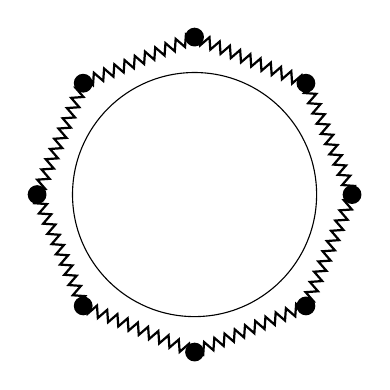
\begin{tikzpicture}[scale=1.0]
  \def\R{2.0}
  \def\rin{1.55}
  \foreach \i in {0,...,7}{
    \coordinate (M\i) at ({90-45*\i}:\R);
  }
  \foreach \i [evaluate=\i as \j using {int(mod(\i+1,8))}] in {0,...,7}{
    \draw[thick,decorate,decoration={zigzag,segment length=4pt,amplitude=2pt}] (M\i) -- (M\j);
  }
  \draw[thin] (0,0) circle (\rin);
  \foreach \i in {0,...,7}{\fill (M\i) circle (3.4pt);}
\end{tikzpicture}
\caption{弹簧振子链}
\label{fig:spring-chain}
\end{figure}

引入向量 $\bm x\equiv(x_1,x_2,\ldots,x_n)^{\mathrm T}$，方程 (1) 可以改写成矩阵形式
\begin{equation}
\ddot{\bm x}+\omega_0^2K\bm x=0,
\tag{2}
\end{equation}
其中 $\omega_0^2\equiv\kappa/m$，对称矩阵
\begin{equation}
K=
\begin{pmatrix}
2&-1&&&-1\\
-1&2&-1&&\\
&-1&\ddots&\ddots&\\
&&\ddots&\ddots&-1\\
-1&&&-1&2
\end{pmatrix}.
\tag{3}
\end{equation}
如果我们能够将矩阵 $K$ 对角化：$K=Q^{\mathrm T}DQ$，上述微分方程可以改写成
\begin{equation}
\left[\frac{d^2}{dt^2}+\omega_0^2D\right]Q\bm x=0,
\tag{4}
\end{equation}
那么，方程对于 $\bm y\equiv Q\bm x$ 而言就变成了一系列独立的一维常微分方程，可以轻松地写下问题的解。所以我们关心的重点就成了矩阵对角化。

\begin{enumerate}
\item 试分别对于 $n=2,16,128,1024$ 的情形，数值求解矩阵 $K$ 的全部本征值。检验它们与如下解析公式相符：
\begin{equation}
\lambda_k=2\left(1-\cos\frac{2\pi k}{n}\right).
\tag{5}
\end{equation}
本征值有如此简单的结构，意味着这个问题可以解析化简：考察本征值方程
\begin{equation}
-x_{j-1}+2x_j-x_{j+1}=\lambda x_j,
\tag{6}
\end{equation}
改写成矩阵形式
\begin{equation}
\begin{pmatrix}x_{j+1}\\x_j\end{pmatrix}
=
\begin{pmatrix}2-\lambda&-1\\1&0\end{pmatrix}
\begin{pmatrix}x_j\\x_{j-1}\end{pmatrix},
\tag{7}
\end{equation}
变成了传输矩阵的形式，我们可以写下
\begin{equation}
\begin{pmatrix}x_{j+n}\\x_{j+n-1}\end{pmatrix}
=
\begin{pmatrix}2-\lambda&-1\\1&0\end{pmatrix}^{n}
\begin{pmatrix}x_j\\x_{j-1}\end{pmatrix}.
\tag{8}
\end{equation}
同矩阵指数一样，矩阵幂的计算也可以转换成求解矩阵本征值问题。记 $c=(2-\lambda)/2$，(7) 式中矩阵的本征值 $\eta$ 满足方程
\begin{equation}
\eta(\eta-2c)+1=0,
\tag{9}
\end{equation}
故
\begin{equation}
\eta_{\pm}=c\pm\sqrt{c^2-1}.
\tag{10}
\end{equation}
代入周期边界条件 $x_k=x_{k+n}$，有
\begin{equation}
\begin{pmatrix}\eta_+^n&0\\0&\eta_-^n\end{pmatrix}=I.
\tag{11}
\end{equation}
要让这个等式成立，必有
\begin{equation}
\eta_+^n=\eta_-^n=1,
\tag{12}
\end{equation}
即 $\eta_{\pm}=\exp(\pm i2\pi k/n)$。相应可以导出前述 $\lambda$ 的解析表达式。

下面，我们来给这个链条加上一些别的约束。给每个振子额外再绑上一根弹簧（见图 3.8），这些额外弹簧的劲度系数呈周期变化。此时，系统的运动方程变为
\begin{equation}
m\ddot x_j=\kappa(x_{j+1}-x_j)+\kappa(x_{j-1}-x_j)-[g_0+g_1\cos(2\pi j\alpha)]x_j,
\qquad j=1,2,\ldots,n.
\tag{13}
\end{equation}
容易检验，此时系统的本征值方程为
\begin{equation}
x_{j+1}=\left[2-\lambda+\frac{g_0+g_1\cos(2\pi j\alpha)}{\kappa}\right]x_j-x_{j-1}.
\tag{14}
\end{equation}
记 $c=(2-\lambda+g_0/\kappa)$，$\gamma=g_1/\kappa$，请求解以下问题：

\begin{figure}[htbp]
\centering
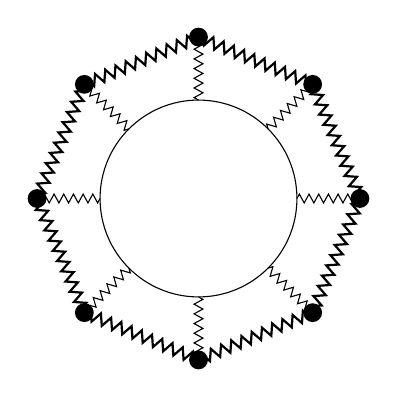
\begin{tikzpicture}[scale=1.0]
  \def\R{2.05}
  \def\rin{1.25}
  \foreach \i in {0,...,7}{
    \coordinate (M\i) at ({90-45*\i}:\R);
    \coordinate (A\i) at ({90-45*\i}:\rin);
  }
  \foreach \i [evaluate=\i as \j using {int(mod(\i+1,8))}] in {0,...,7}{
    \draw[thick,decorate,decoration={zigzag,segment length=4pt,amplitude=2pt}] (M\i) -- (M\j);
  }
  \draw[thin] (0,0) circle (\rin);
  \foreach \i in {0,...,7}{
    \draw[thin,decorate,decoration={zigzag,segment length=3.5pt,amplitude=1.6pt}] (A\i) -- (M\i);
    \fill (M\i) circle (3.4pt);
  }
\end{tikzpicture}
\caption{有约束的弹簧振子链}
\label{fig:constrained-spring-chain}
\end{figure}

\item 取 $\gamma=2,\alpha=1/2,n=720$，直接对角化矩阵 $K$，求解其全部本征值。请检验，$c$ 分布在两个分立的区间中。本征谱的这种分离在凝聚态物理中相当常见，有时叫作电子的价带和导带，有时又称为声子的声学支和光学支。
\item 仿照题文中的操作，检验本征谱可以通过分析从 $(x_j,x_{j-1},x_{j-2})^{\mathrm T}$ 到 $(x_{j+2},x_{j+1},x_j)^{\mathrm T}$ 的传输矩阵给出。用你得到的解析表达式验证数值结果。
\item 分别对于 $\alpha=1/3,1/4$，给出 $c$ 的容许区间。此时无须考虑 $n$ 的限制。
\item 给出更多的算例，检验对于任意 $\alpha=p/q\in(0,1)$，其中 $p,q$ 互素，本征谱的容许区间会劈裂成 $q$ 份。
\item 给定 $\gamma=2,n=720$，连续变化 $\alpha$，请在 $\alpha$--$c$ 平面上画出全体本征值的散点图。检验你看到了一只“蝴蝶”。
\end{enumerate}

本题中 (14) 式被称为 Harper 方程，最初从分析二维晶格在均匀外磁场下的能带总结而来：无量纲参数 $\alpha$ 对应于晶格元胞磁通量与磁通量子 $hc/e$ 之比；本征谱的分裂与磁性 Bloch 能带以及整数数量子霍尔效应中的拓扑能隙结构密切相关；而那只“蝴蝶”被称为 Hofstadter 蝴蝶。对于无理数 $\alpha$ 且非零调制强度，能谱为 Cantor 集这一“Ten Martini Problem”后来已经得到严格证明。\jiaokan{原文称本征谱劈裂“对应于分数阶量子霍尔效应”，并称无理 $\alpha$ 时能谱为 Cantor 集“尚未得到严格证明”。前者容易与依赖电子相互作用的分数量子霍尔效应混淆：Harper/Hofstadter 单粒子模型的能隙与整数数量子霍尔效应及 陈数（Chern number）所刻画的拓扑结构直接相关。后者亦已过时；Avila 与 \rusname{Житомирская} 在 2009 年解决 Ten Martini Problem，证明 almost Mathieu 算子在无理频率和非零耦合下的谱为 Cantor 集。}

% R09 extends through the end of Chapter 3 (source PDF page 145 / printed page 130).
